%%%%%%%%%%%%%%%%%%%%%%%%%%%%%%%%%%%%%%%%%%%%%%%%%%%%%%
% A Beamer template for University of Wollongong     %
% Based on THU beamer theme                          %
% Author: Qiuyu Lu                                   %
% Date: July 2024                                    %
% LPPL Licensed.                                     %
%%%%%%%%%%%%%%%%%%%%%%%%%%%%%%%%%%%%%%%%%%%%%%%%%%%%%%
% Customized for Sharif University of Technology     %
%%%%%%%%%%%%%%%%%%%%%%%%%%%%%%%%%%%%%%%%%%%%%%%%%%%%%%


\documentclass[serif, aspectratio=169]{beamer}
%\documentclass[serif]{beamer}  % for 4:3 ratio
\usepackage[T1]{fontenc} 
\usepackage{fourier} % see "http://faq.ktug.org/wiki/uploads/MathFonts.pdf" for other options
\usepackage{hyperref}
\usepackage{latexsym,amsmath,xcolor,multicol,booktabs,calligra}
\usepackage{graphicx,pstricks,listings,stackengine}
\usepackage{lipsum}
\usepackage{array}
\usepackage{tikz}
\usepackage{tcolorbox}
\usepackage{graphicx}
\usepackage{amsfonts}
\usepackage{hyperref}


\usetikzlibrary{positioning,calc}





\author{Ali Sharifi-Zarchi}
\title{Machine Learning (CE 40717)}
\subtitle{Fall 2024}
\institute{
    CE Department \\
    Sharif University of Technology
}
%\date{\small \today}
% \usepackage{UoWstyle}
\usepackage{SUTstyle}

% defs
\def\cmd#1{\texttt{\color{red}\footnotesize $\backslash$#1}}
\def\env#1{\texttt{\color{blue}\footnotesize #1}}
\definecolor{deepblue}{rgb}{0,0,0.5}
\definecolor{deepred}{RGB}{153,0,0}
\definecolor{deepgreen}{rgb}{0,0.5,0}
\definecolor{halfgray}{gray}{0.55}


% Define custom colors
\definecolor{blue!20}{RGB}{173, 216, 230}
\definecolor{green!20}{RGB}{144, 238, 144}
\definecolor{red!20}{RGB}{255, 182, 193}

\lstset{
    basicstyle=\ttfamily\small,
    keywordstyle=\bfseries\color{deepblue},
    emphstyle=\ttfamily\color{deepred},    % Custom highlighting style
    stringstyle=\color{deepgreen},
    numbers=left,
    numberstyle=\small\color{halfgray},
    rulesepcolor=\color{red!20!green!20!blue!20},
    frame=shadowbox,
}


\begin{document}

\begin{frame}
    \titlepage
    \vspace*{-0.6cm}
    \begin{figure}[htpb]
        \begin{center}
            
\includegraphics[keepaspectratio, scale=0.25]{pic/sharif-main-logo.png}
        \end{center}
    \end{figure}
\end{frame}

\begin{frame}    
\tableofcontents[sectionstyle=show,
subsectionstyle=show/shaded/hide,
subsubsectionstyle=show/shaded/hide]
\end{frame}


\section{Autoencoder Fundamentals}

\begin{frame}{Unlabeled Data Usage in Deep Learning}
\begin{center}
    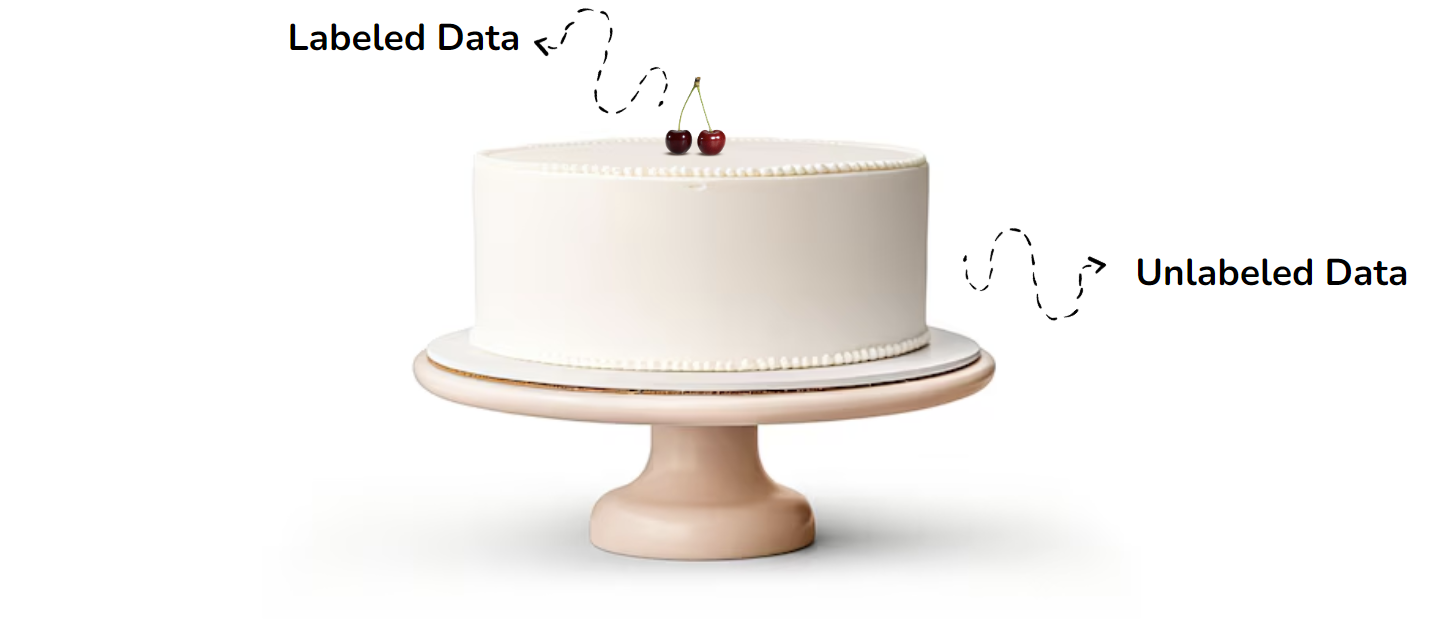
\includegraphics[width=0.8\textwidth]{pic/Cherry on top.png}
    \\
    \textbf{How can we use unlabeled data in our deep neural networks?}

    \vfill
    \hspace*{-1\textwidth}{\scriptsize Image: \href{https://www.freepik.com/premium-ai-image/plain-white-cake-stand-isolated-white-background-round-cake-mockup_75039828.htm}{Source}}

\end{center}
    
\end{frame}

\begin{frame}{What Is Latent Variable?}
    \begin{itemize}
        \item \textbf{Definition:} Latent variables are variables that are not directly observed but are inferred from other variables that are observed (measured).
    \end{itemize}
    
    \vspace{0.5cm} % Adjust the space as needed
    
    \begin{itemize}
        \item \textbf{Origin:} Derived from the Latin word \textit{latēre} meaning "hidden".
    \end{itemize}

    \vspace{0.5cm} % Adjust the space as needed
    
    \begin{itemize}
        \item \textbf{Examples:}
        \begin{itemize}
            \item Personality traits (in psychology)
            \item Economic factors like inflation (in economics)
            \item Topic of a document (in natural language processing)
        \end{itemize}
    \end{itemize}

\end{frame}

\begin{frame}{What Is Latent Variable?}
      \begin{center}
        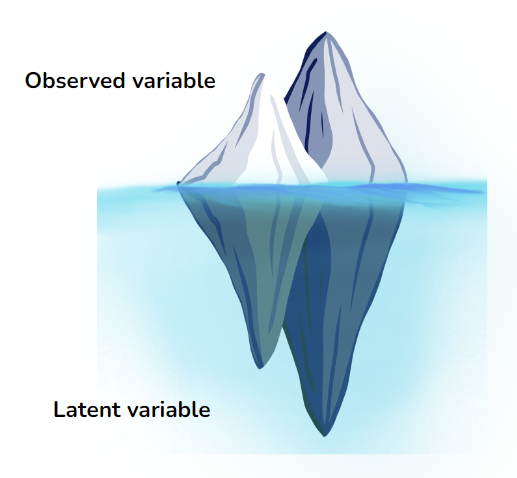
\includegraphics[width=0.5\textwidth]{pic/what is latent variable.png} 
    \end{center}
\end{frame}


\begin{frame}{Latent Variables in Deep Learning}
        \textbf{We can train \textcolor{blue}{deep neural networks} using  \textcolor{blue}{unlabeled data} to infer \textcolor{blue}{latent variables} in order to:}
        \vspace{0.5cm}
        \begin{itemize}
        \small
            \item Compress data
            \item Generate new data
            \item Denoise Data
            \item Using latent variables as features for various tasks like classification
            \item ...
        \end{itemize}
\end{frame}


\begin{frame}{Autoencoder: Background}
    \begin{center}
        \textbf{Using latent variables as a foundation}, an unsupervised approach for learning a lower-dimensional feature representation from unlabeled training data.
        
        \vspace{0.3cm}
        
        \begin{minipage}{0.6\textwidth}
            \centering
            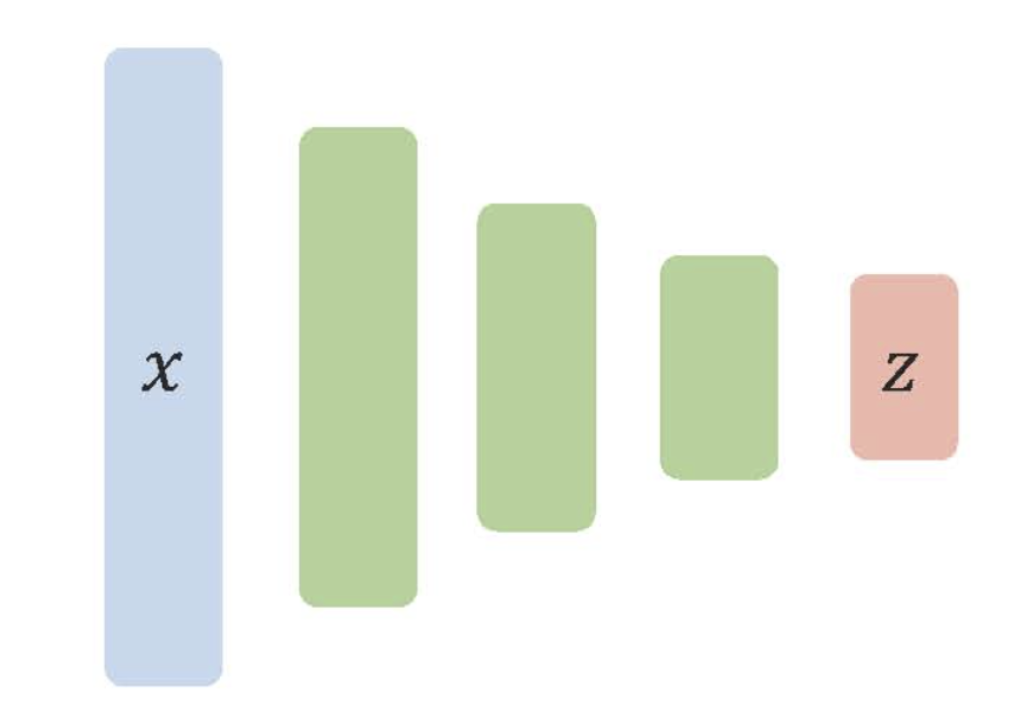
\includegraphics[width=0.7\textwidth]{pic/AE background1.png}
        \end{minipage}
        \hspace{0.05\textwidth} 
        \begin{minipage}{0.3\textwidth}
            \raggedright
            Why do we care about a \\ low-dimensional \textit{$z$}?
        \end{minipage}
        
        \vspace{0.3cm}
        
        \textit{"Encoder"} learns mapping from the data, \textit{$x$}, to a low-dimensional latent space, \textit{$z$}
    \end{center}
\end{frame}

\begin{frame}{Autoencoders: Background}

    How can we learn this latent space? \\
    Train the model to use these features to \textbf{reconstruct the desired (usually original) data}.


    \begin{center}
                
        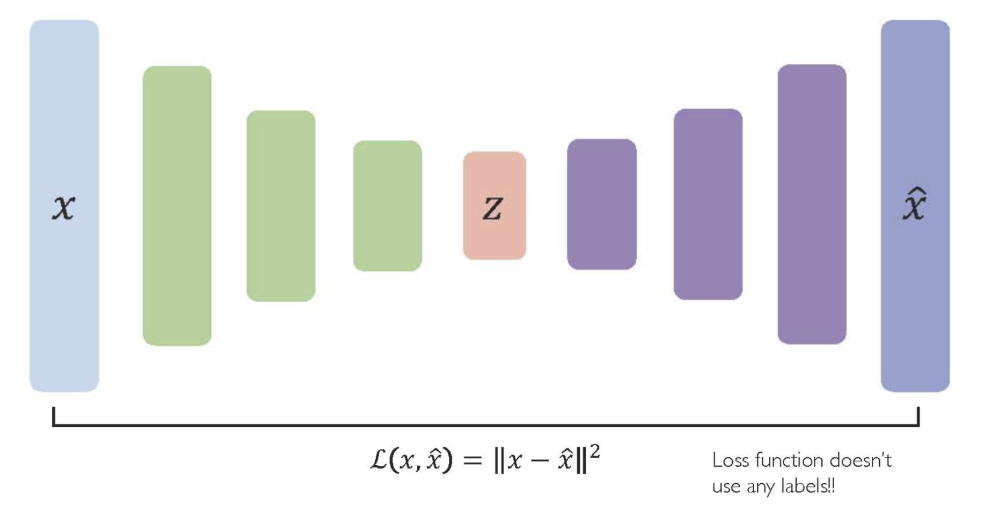
\includegraphics[width=0.7\textwidth]{pic/AE background2.png} 

        
        \textit{"Decoder"} learns mapping back from latent \textit{z}, to a reconstructed observation, \textit{x}
    \end{center}
\end{frame}

\begin{frame}{Autoencoders}
    \begin{enumerate}
        \item These models map between \textbf{\textcolor{deepblue}{observation space $\mathbf{x} \in \mathbb{R}^D$}} and \textbf{\textcolor{deepblue}{latent space $\mathbf{z} \in \mathbb{R}^Q$}}:
        
        \begin{itemize}
            \item \textbf{\textcolor{deepblue}{Encoder}} \quad \( f_w  :  \mathbf{x} \mapsto \mathbf{z} \)   \hspace{em} {\tiny{The "Analysis" net which computes the hidden representation}}
            \item \textbf{\textcolor{deepblue}{Decoder}} \quad \( g_w : \mathbf{z} \mapsto \mathbf{x} \)   \hspace{em} {\tiny{The "Synthesis" which recomposes the data from the hidden representation}}
        \end{itemize}
        
        \vspace{0.3cm}

        \item Models are linear or non-linear, deterministic or stochastic, with/without encoder.
    \end{enumerate}
    
    
    \begin{center}
\        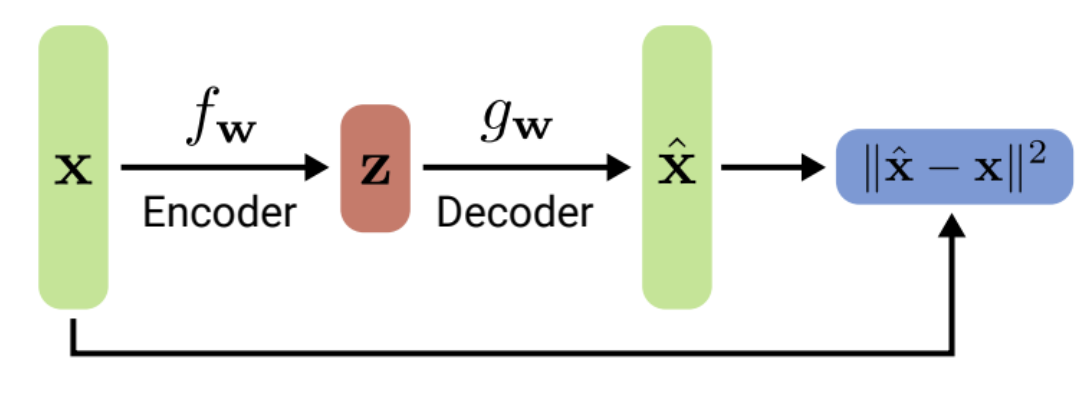
\includegraphics[width=0.8\textwidth]{pic/AE1.png}\
    \end{center}
\end{frame}

\begin{frame}{Autoencoder Without a Non-linearity}
    
    \begin{center}
        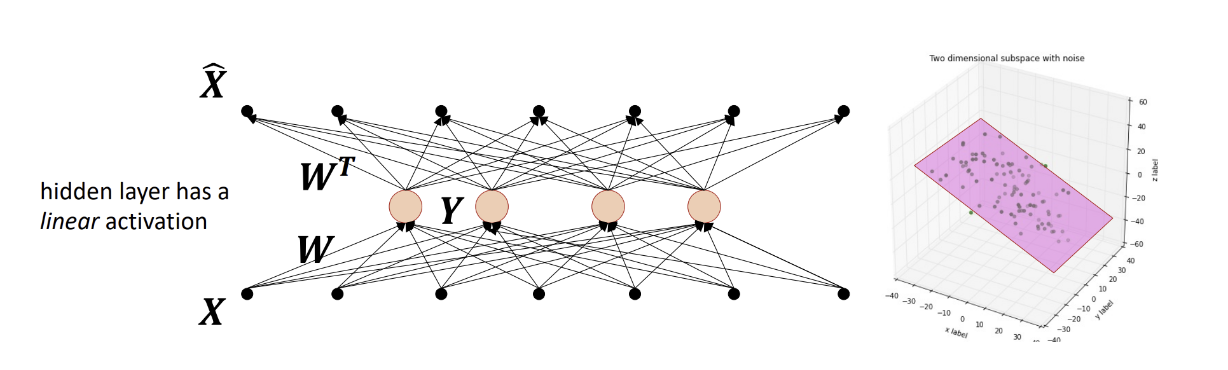
\includegraphics[width=0.85\textwidth]{pic/AE without non-linearity.png}
    \end{center}
    
    
\begin{center}
    \fbox{\textbf{\textcolor{deepblue}{\(\mathbf{Y = WX} \)}}} \hspace{0.5cm} 
    \fbox{\textbf{\textcolor{deepblue}{\(\hat{\mathbf{X}} = W^{T} \mathbf{Y}\)}}} \hspace{0.5cm}
    \textbf{\textcolor{deepred}{\( E = \| \mathbf{X} - W^{T} W \mathbf{X} \|^2 \)}} \hspace{0.5cm}
    \footnotesize{Find \(W\) to minimize \(\text{Avg}[E]\)}
\end{center}

        
    \begin{itemize}
        \item \textbf{This is similar to PCA}
        \item[] \textendash \ The output of the hidden layer will be in the principal subspace
        \begin{itemize}
            \item[] \textbullet \ Even if the recomposition weights are different from the "analysis" weights
        \end{itemize}
    \end{itemize}
\end{frame}

\begin{frame}{``Deep'' AE}
    \begin{itemize}
        \item \textbf{Deep nonlinear autoencoders} learn to project the data, not onto a subspace, but onto a nonlinear \textcolor{deepgreen}{manifold}.
        \vspace{0.1cm}
        
        \item This manifold is the \textbf{image of the decoder}.
        \vspace{0.1cm}
        
        \item This is a kind of \textcolor{deepgreen}{nonlinear dimensionality reduction}.
    \end{itemize}
    
    
    \begin{center}
        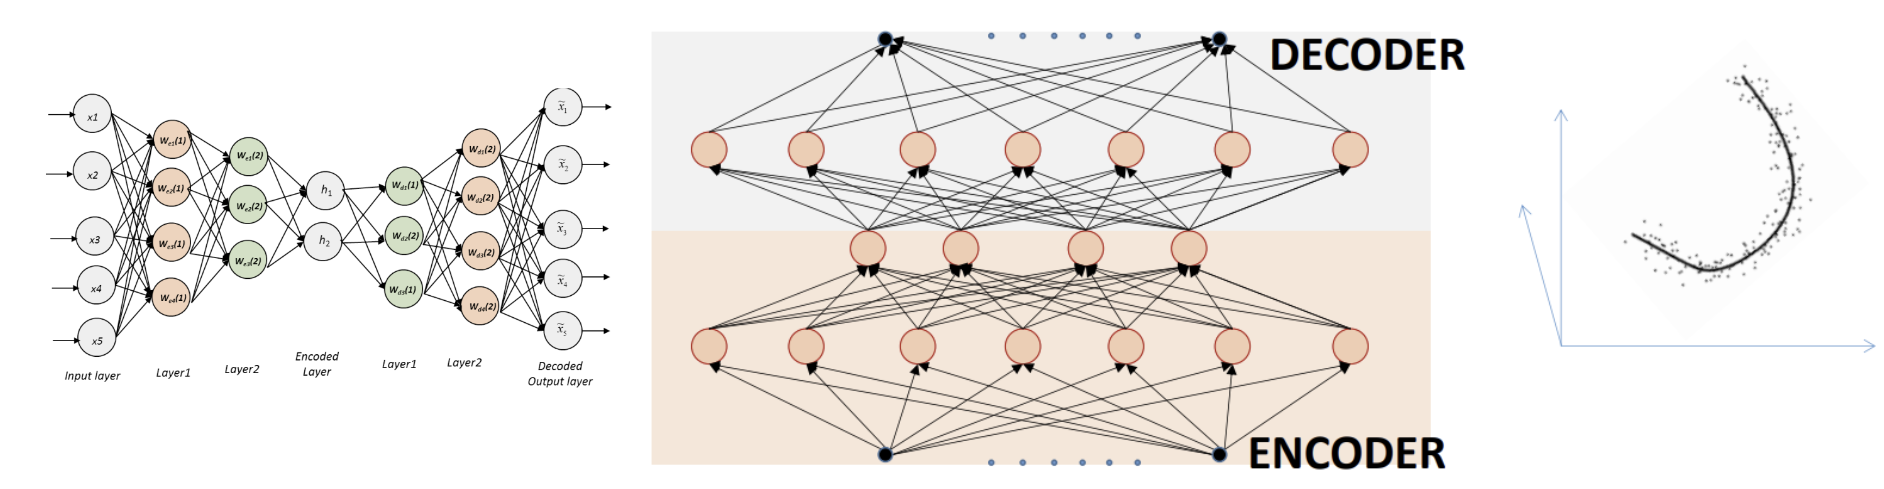
\includegraphics[width=\textwidth]{pic/Deep AE1.png} 
    \end{center}
    
\end{frame}

\begin{frame}{AE vs PCA}
    As we said, \textbf{PCA} can be described as
    \begin{center}
        \begin{minipage}{0.6\textwidth}
            \begin{center}
                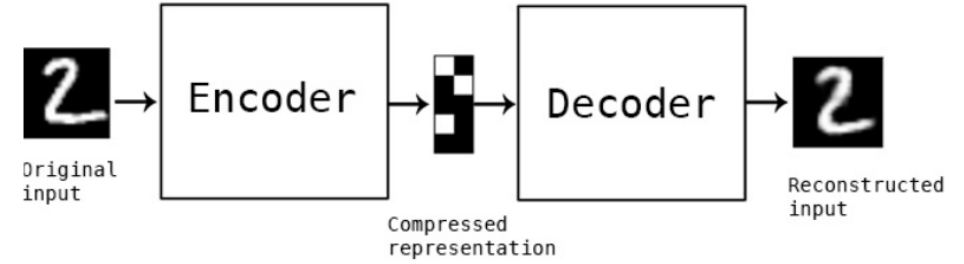
\includegraphics[width=\textwidth]{pic/AE vs PCA 1.png}
            \end{center}
        \end{minipage}
        \hfill
        \begin{minipage}{0.35\textwidth}
            \begin{align*}
                &\min_{W} \sum \| \hat{x} - x \|^2 \\
                &W^T W = I \\
                &\min_{W} \sum \| W^T W x - x \|^2
            \end{align*}
        \end{minipage}
        
        \vspace{0.3cm}
    \end{center}
    And also \textbf{Autoencoders} can be thought of as a \textbf{non-linear PCA}.
    \begin{center}                
        \begin{minipage}{0.6\textwidth}
            \begin{center}
                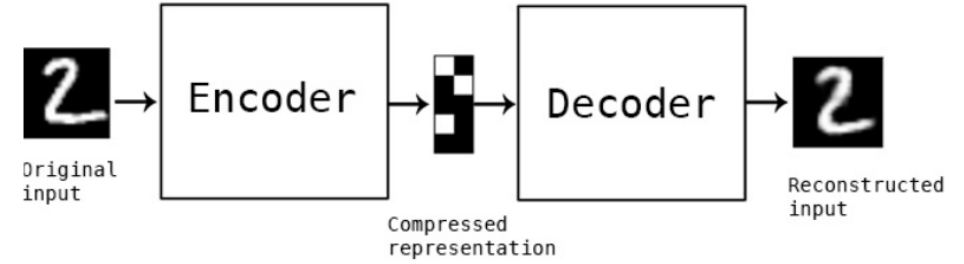
\includegraphics[width=\textwidth]{pic/AE vs PCA 1.png} 
            \end{center}
        \end{minipage}
        \hfill
        \begin{minipage}{0.35\textwidth}
            \begin{align*}
                &\min_{h, g} \sum \| \hat{x} - x \|^2 \\
                &\min_{h, g} \sum \| g(f(x)) - x \|^2
            \end{align*}
        \end{minipage}
    \end{center}
\end{frame}

\begin{frame}{AE vs PCA}

    Nonlinear autoencoders can learn more powerful codes for a given dimensionality, compared with linear autoencoders (PCA).
    
    
    % Centered image
    \begin{center}
        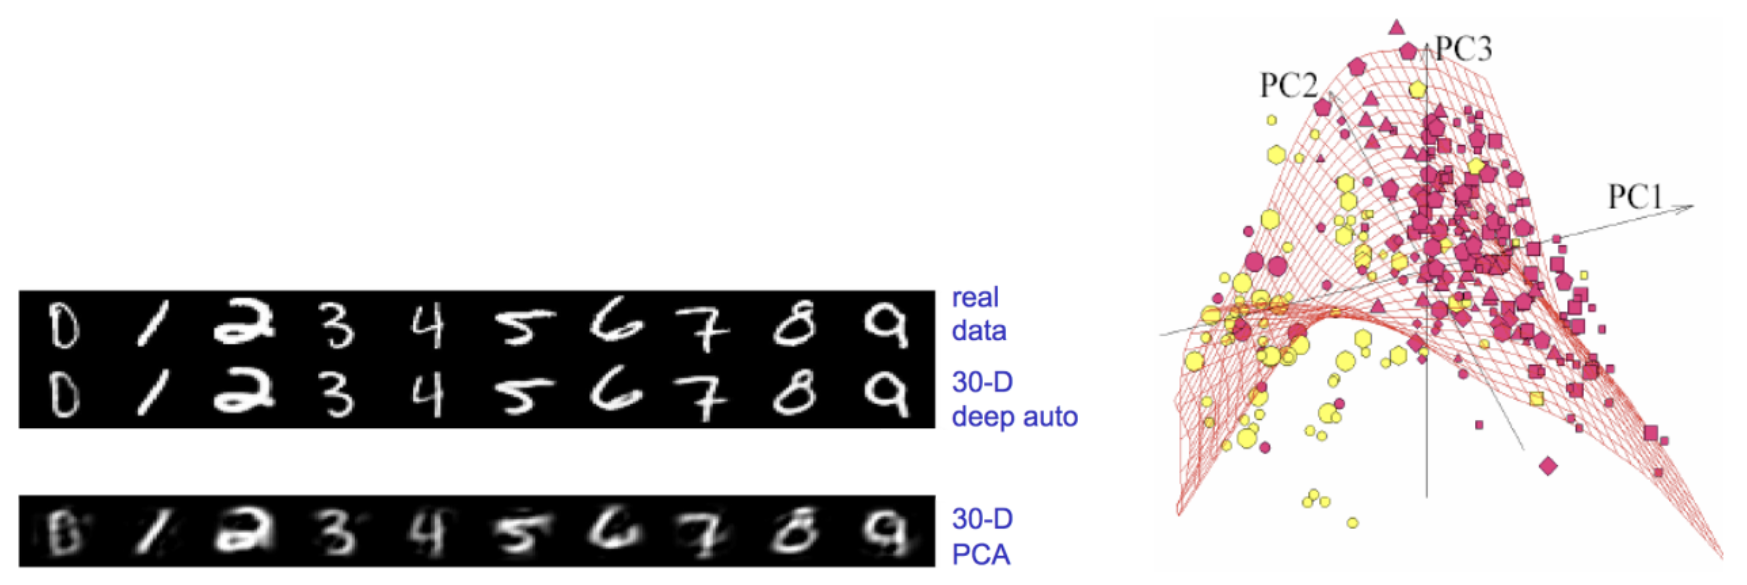
\includegraphics[width=\textwidth]{pic/AE vs PCA 2.png} 
    \end{center}
\end{frame}


\begin{frame}{Autoencoder Key Characteristics}
\small
     
    \begin{itemize}
        \item \textbf{Specialized for Specific Data Type}
        \begin{itemize}
            \item Autoencoders excel at recognizing patterns in the type of data they were trained on, but may fail on different data types.
            \item Example: A model trained on animal images will not perform well when applied to landscapes.
        \end{itemize}
        
        \vspace{0.25cm}
        
        \item \textbf{Tailored Compression vs. General Algorithms}
        \begin{itemize}
            \item Unlike generic compression techniques (MP3, JPEG), which apply universal rules, autoencoders customize their approach to fit the training data structure.
        \end{itemize}
        
        \vspace{0.25cm}
        
        \item \textbf{Loss of Detail in Output}
        \begin{itemize}
            \item Autoencoders don’t retain all the original information, leading to some degradation in the reconstructed data.
            \item This makes them "lossy" – similar to formats like MP3 or JPEG, which prioritize size over perfect fidelity.
        \end{itemize}
    \end{itemize}
    

\end{frame}


\begin{frame}{Fully Convolutional AE}
    \begin{center}
        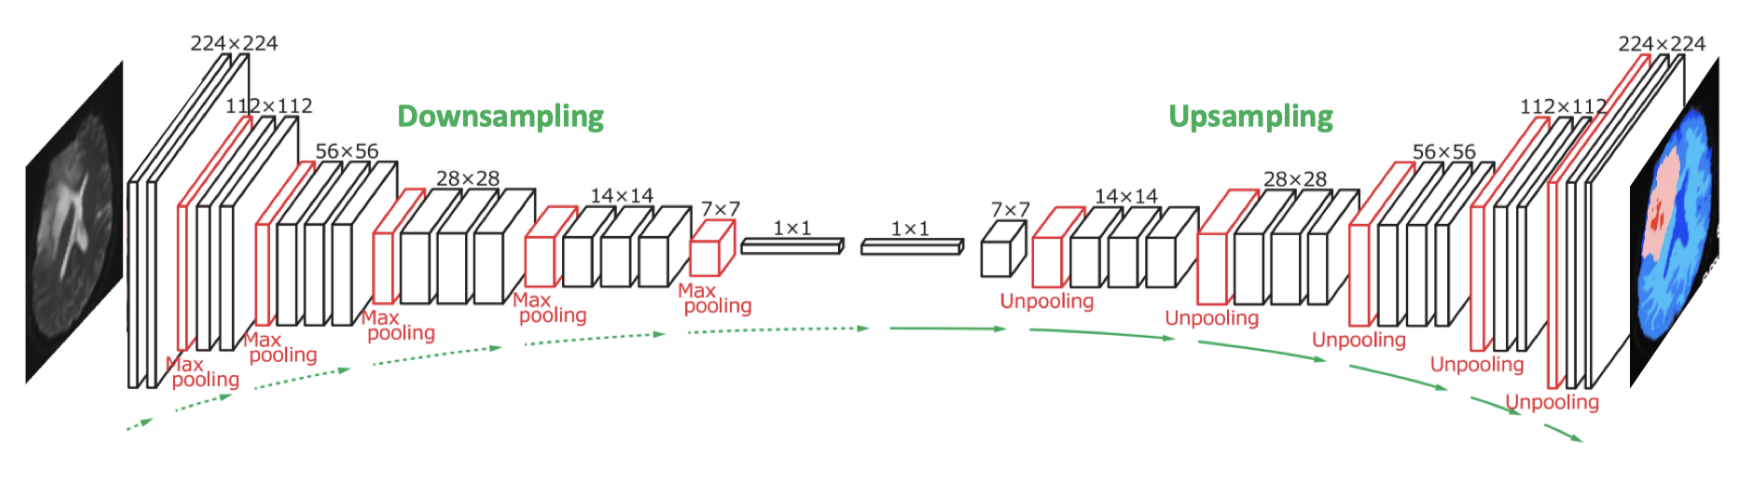
\includegraphics[width=\textwidth]{pic/Fully Convolutional AE 1.png} 
    \end{center}
    
    \vspace{0.5cm}
    
    \begin{center}
        We will discuss more about \textbf{"Downsampling"} and \textbf{"Upsampling"} in the next section
    \end{center}
    
    \vspace{1cm}
    
    % Image credit
    \tiny{Image from \href{https://mriquestions.com/upsampling.html}{this link}}
\end{frame}

\begin{frame}{Autoencoders As Pretrained Models}
    \scriptsize
    \begin{itemize}
        \item \textbf{Feature Extraction:} Encoder \textbf{learns} data patterns and \textbf{compresses} them into useful features.
        \item \textbf{Supervised Model Initialization:} Use the \textbf{pretrained encoder} to initialize a supervised learning model.
        \item \textbf{Fine-Tuning:} Train the encoder and classifier \textbf{together} to improve performance.
        \item \textbf{Useful with Small Data:} Effective when training on \textbf{small datasets} by leveraging pretrained features.
    \end{itemize}
    
    \begin{center}
        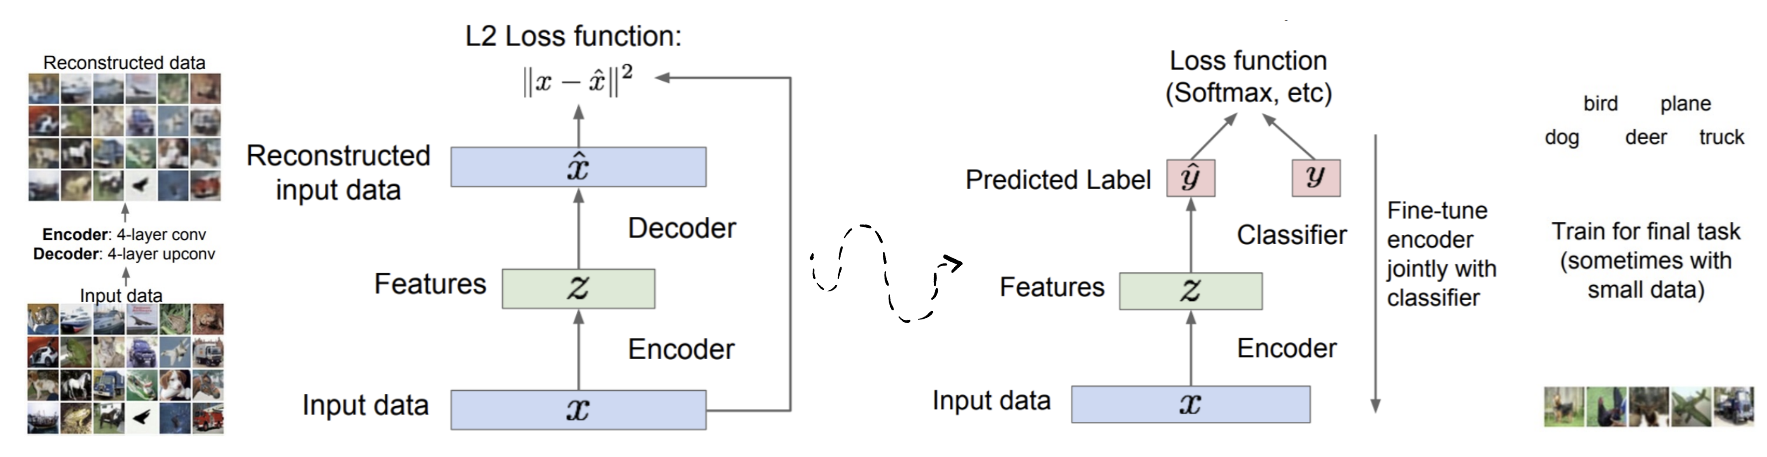
\includegraphics[width=0.9\textwidth]{pic/AEs as pretrained models.png} 
    \end{center}
\end{frame}

\begin{frame}{AE Performance \& Bottleneck Size (MNIST Example)}
    \begin{itemize}
        \item \textbf{Reconstruction Error and Bottleneck Size:}
        \begin{itemize}
            \item A good autoencoder should minimize reconstruction error.
            \item The error depends heavily on the size of the \( z \) (the dimension of the latent space).
        \end{itemize}
        
        \item \textbf{Experiment Setup:}
        \begin{itemize}
            \item CNN-based AE trained on MNIST with different bottleneck sizes:
            \begin{itemize}
                \item \((2, 1, 1)\), \((4, 1, 1)\) \& \((32, 1, 1)\)
            \end{itemize} 
        \end{itemize}
    \end{itemize}
\end{frame}

\begin{frame}{AE Performance \& Bottleneck Size (MNIST Example) - Results}
    \begin{columns}[t] 
        \begin{column}{0.65\textwidth} 
            \begin{itemize}
                \item \textbf{Results:}
                \begin{itemize}
                \footnotesize
                    \item With \( d=2 \): Reconstruction is still good; a classifier could identify digits decently.
                    \item With \( d=32 \): Reconstruction is nearly perfect; despite a compression ratio of \(\sim0.04\) (from 32 to 28x28).
                \end{itemize}
                \vspace{1cm}
                \item \textbf{Larger latent spaces} generally lead to \textbf{better reconstructions}, as more variables allow more information to be preserved during compression.
            \end{itemize}
        \end{column}
        
        % Right column with image
        \begin{column}{0.4\textwidth}% Adjust the width for better fit
            \vspace{-1.5cm}
            \begin{center}
                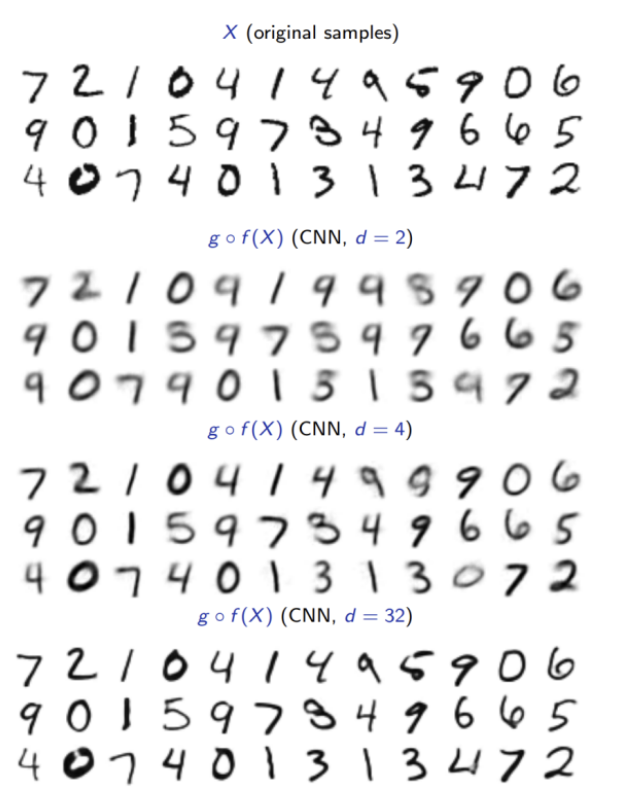
\includegraphics[width=\textwidth, height=\textheight, keepaspectratio]{pic/AE Performance & Bottleneck Size (MNIST Example).png} 
                    \vspace{2.5cm}
            \end{center}
        \end{column}
    \end{columns}
\end{frame}

\section{Types of Autoencoders}

\begin{frame}{AE’s: Undercomplete Autoencoders}
    \begin{enumerate}
        \item An autoencoder whose code dimension is less than the input dimension is called \textcolor{blue}{undercomplete}.
        \vspace{0.3cm}
        
        \item Learning an undercomplete representation forces the autoencoder to capture the most salient features of the training data.
        \vspace{0.3cm}
        
        \item The learning process is described simply as minimizing a loss function
        \begin{equation*}
            L(x, g(f(x)))
        \end{equation*}
        where \( L \) is a loss function penalizing \( g(f(x)) \) for being dissimilar from \( x \), such as the mean squared error.
    \end{enumerate}
\end{frame}

\begin{frame}{AE’s: Overcomplete Autoencoders}
\small
    \begin{enumerate}
        \item \textcolor{black}{consider encoder} \textit{\textcolor{blue}{f}} \textcolor{black}{and decoder} \textit{\textcolor{blue}{g}}.
        
        \begin{equation*}
            X \in \mathbb{R}^d \quad h \in \mathbb{R}^k
        \end{equation*}
        
        \vspace{0.15cm}
        \item When \( k > d \), the autoencoder is called \textcolor{blue}{Overcomplete Autoencoders}.
        
        \vspace{0.2cm}
        \item There are other ways we can constrain the reconstruction of an autoencoder than to impose a hidden layer of smaller dimension than the input.
        
        \vspace{0.2cm}
        \item Regularized Autoencoders use a loss function that encourages the model to have some properties besides reproducing inputs.
        \begin{itemize}
            \item Sparsity representation (Sparse Autoencoders)
            \item Smallness of derivative of representation (Contractive Autoencoders)
            \item Robustness to noise or to missing inputs (Denoising Autoencoders)
        \end{itemize}
    \end{enumerate}
\end{frame}


\begin{frame}{AE’s: Sparse Autoencoders (Intuition)}
    \scriptsize
    
    \textbf{Idea:} Can we describe the input with a small set of \textit{“attributes”?}
    \\\textbf{This might be a more \textit{compressed} and \textit{structured} representation.}
    
    \begin{columns}[t]
    
        % Left Column
        \begin{column}{0.7\textwidth}
        
             \textbf{\textcolor{deepgreen}{1. NOT structured}} - \textit{“dense”: most values non-zero}
            % Dense Representation Example - Row Layout
            \begin{tcolorbox}[colback=white!10, colframe=white, boxrule=0.5pt, width=\textwidth]
                \begin{columns}[T]
                    \begin{column}{0.2\textwidth}
                        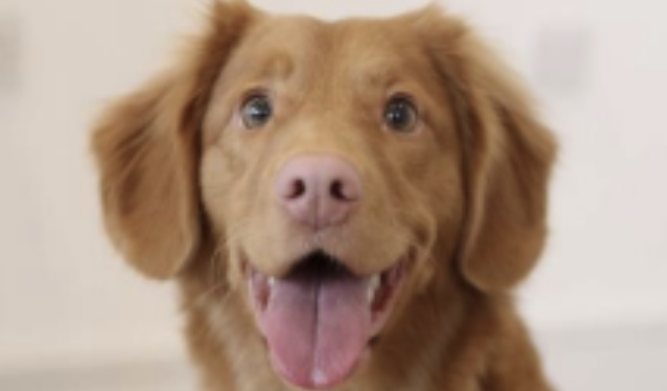
\includegraphics[width=\textwidth]{pic/SAE dog.png} 
                    \end{column}
                    \begin{column}{0.75\textwidth}
                        \scriptsize{\texttt{Pixel (0,0): \#FE057D \\
                        Pixel (0,1): \#FD0263 \\
                        Pixel (0,2): \#E1065F}} \\
                    \end{column}
                \end{columns}
            \end{tcolorbox}

            
        \vspace{0.3cm}

            \textbf{\textcolor{deepred}{Idea: “Sparse” representations are going to be more structured!}}
            
        \vspace{0.6cm}

            % Sparse Representation Example - Row Layout
            \textbf{\textcolor{deepgreen}{2. Very structured!}} - \textit{“sparse”: most values are zero}
            \begin{tcolorbox}[colback=white!10, colframe=white, boxrule=0.5pt, width=0.7\textwidth]
                \begin{columns}[T]
                \hspace{0.5cm}
                    \begin{column}{0.3\textwidth}
                        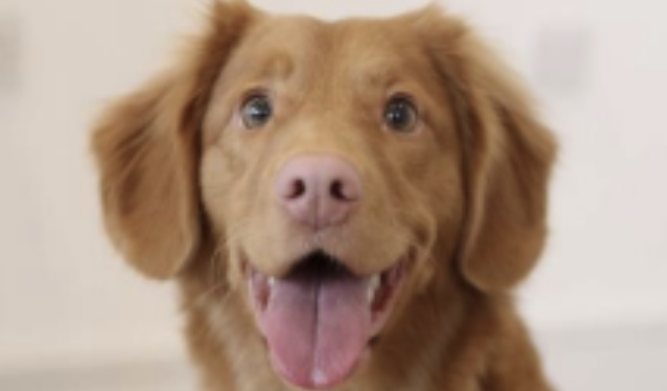
\includegraphics[width=\textwidth]{pic/SAE dog.png} 
                    \end{column}
                    \begin{column}{0.75\textwidth}
                        \scriptsize{\texttt{has\_ears: 1 \\
                        has\_wings: 0 \\
                        has\_wheels: 0}} \\
                    \end{column}
                \end{columns}
            \end{tcolorbox}
            
 
        \end{column}
        
        % Right Column - Aside
        \begin{column}{0.4\textwidth}
        \vspace{-1.3cm}

            \begin{tcolorbox}[colback=blue!5, colframe=blue!70!black, boxrule=0.5pt, width=\textwidth, title=\textbf{Aside:}]
                \scriptsize{This idea originated in neuroscience, where researchers believe that the brain uses \textbf{sparse} representations (see “sparse coding”).}
            \end{tcolorbox}
        \end{column}
        
    \end{columns}
        \vspace{0.2cm}
       \scriptsize{There are many possible “attributes,”\& most images don’t have most of the attributes.}

\end{frame}


\begin{frame}{AE's: Sparese Autoencoder (Big Picture)}
    \begin{center}
        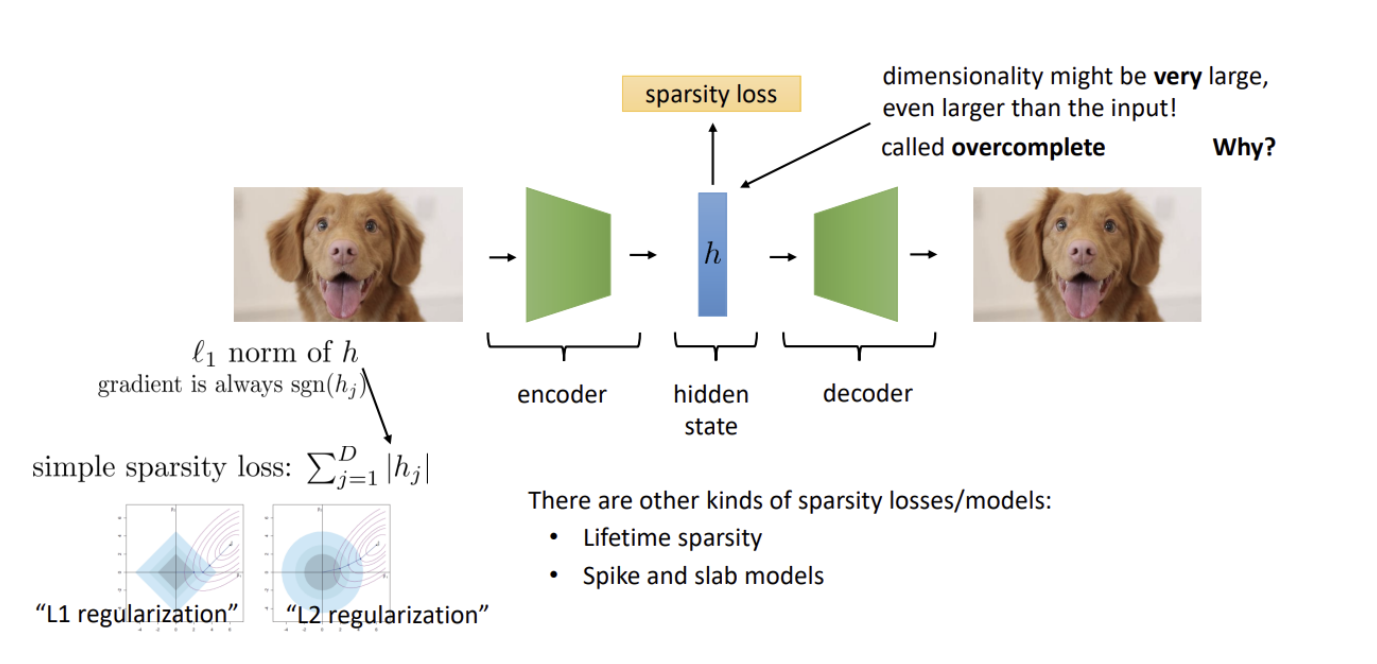
\includegraphics[width=\textwidth]{pic/SAE big picture.png}
    \end{center}

\end{frame}

\begin{frame}{AE’s: Sparse Autoencoders (Details)}
    \vspace{-0.2cm}

    \begin{enumerate}
        \item Sparse Autoencoders try to minimize the following function.
        \[
            L(x, g(f(x))) + \Omega(h)
        \]
        \item The first term is loss for copying inputs.
        \item The second term is sparsity penalty.
        \item In general neural networks, we are trying to find the \textcolor{green!70!black}{\textbf{maximum likelihood:}} \( p(x|\theta) \).
        \item We often use \( \log p(x|\theta) \) for simplification, from which we can get the loss function without regularization.
        \item What about MAP (Maximum a posteriori)?
        \[p(\theta|x) \propto p(x|\theta) \times p(\theta)\]
        \item Maximizing the log of the above function yields:
        \[
            \text{maximize} \ (\log p(x|\theta) + \log p(\theta))
        \]
        \item The first term is the loss function, and the second term is the 
        regularization penalty.
    \end{enumerate}
    \vspace{0.4cm}
\end{frame}


\begin{frame}{AE’s: Denoising Autoencoders (Intuition)}
    \textbf{Idea:} a good model that has learned meaningful structure should “fill in the blanks”
    \hspace{0.3cm}

    \begin{center}
        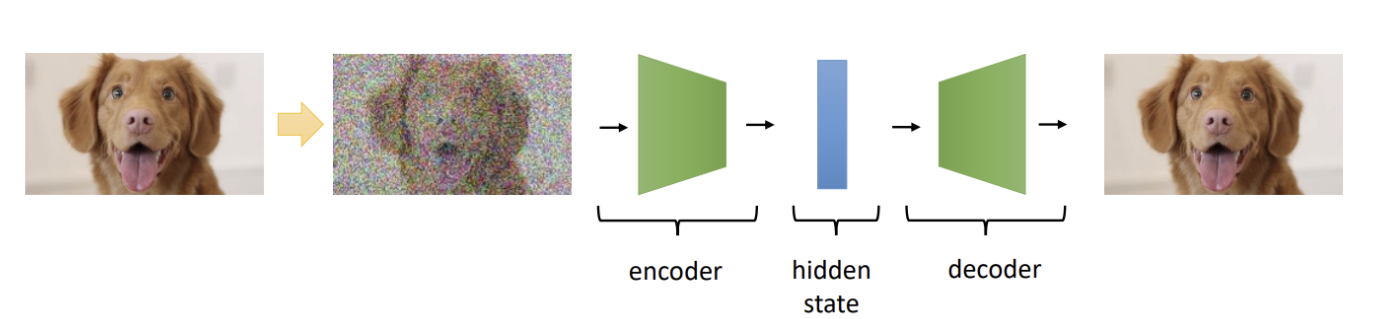
\includegraphics[width=\textwidth]{pic/DAE intuition.png} 
    \end{center}

    \vspace{0.5cm}
        \begin{tcolorbox}[colback=blue!5, colframe=blue!70!black, boxrule=0.5pt, width=0.9\textwidth, sharp corners=south]
        \textbf{There are \textcolor{blue}{many variants} on this basic idea, and this is one of the most widely used simple autoencoder designs.}
    \end{tcolorbox}

\end{frame}


\begin{frame}{AE’s: Denoising Autoencoders (Details)}
    \small
    \vspace{-0.2cm}

    \begin{enumerate}
        \item \textbf{The denoising autoencoder (DAE)} is an autoencoder that receives a corrupted data point as input and is trained to predict the original, uncorrupted data point as its output.
        
        \item \textbf{Traditional autoencoders minimize} {\color{blue} \( L(x, g(f(x))) \)}
        \begin{itemize}
            \item \small \( L \) is a loss function penalizing \( g(f(x)) \) for being dissimilar from \( x \), such as \( L_2 \) norm of difference: mean squared error.
        \end{itemize}

        \item \textbf{A DAE minimizes} {\color{blue} \( L(x, g(f(\tilde{x}))) \)}
        \begin{itemize}
            \item \small \( \tilde{x} \) is a copy of \( x \) that is corrupted by some form of noise.
            \item \small The autoencoder must undo this corruption rather than simply copying their input.
        \end{itemize}
    \end{enumerate}
    
    \vspace{0.3cm}
    \begin{center}
        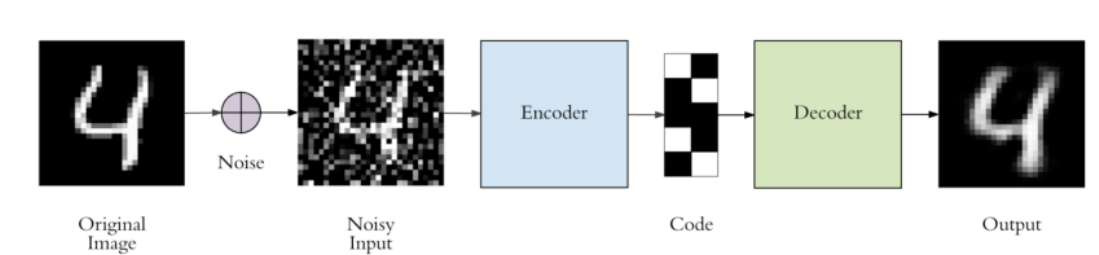
\includegraphics[width=0.7\textwidth]{pic/DAE details1.png}
    \end{center}
\end{frame}



\begin{frame}{AE’s: Denoising Autoencoders (Training Procedure)}
    \small
    \vspace{-0.3cm}
    \begin{enumerate}
        \item The DAE training procedure is
        \begin{center}
            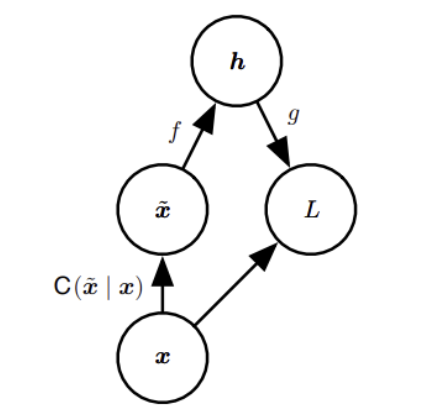
\includegraphics[width=0.3\textwidth]{pic/DAE training.png} 
        \end{center}
        
        \item We introduce a corruption process \( \textcolor{blue}{C(\tilde{x} | x)} \).
    \end{enumerate}
    \vspace{0.3cm}
\end{frame}

\begin{frame}{AE’s: Denoising Autoencoders (Training Procedure)}
    \small
    \vspace{-0.2cm}
    \begin{enumerate}
        \item We introduce a corruption process \( \textcolor{blue}{C(\tilde{x} | x)} \).
        \item The autoencoder then learns a reconstruction distribution \( \textcolor{blue}{p_{\text{reconstruct}}(x | \tilde{x})} \) estimated from training pairs \( \textcolor{blue}{(x, \tilde{x})} \) as follows:
        \begin{itemize}
            \item Sample a training example \( \textcolor{blue}{x_i} \) from the training data.
            \item Sample a corrupted version \( \textcolor{blue}{\tilde{x}_i} \) from \( \textcolor{blue}{C(\tilde{x}_i | x = x_i)} \).
            \item Use \( \textcolor{blue}{(x, \tilde{x})} \) as a training example for estimating the autoencoder reconstruction distribution \( \textcolor{blue}{p_{\text{reconstruct}}(x|\tilde{x}) = p_{\text{decoder}}(x|h)} \) with \( \textcolor{blue}{h} \) the output of encoder \( \textcolor{blue}{f(\tilde{x})} \) and \( \textcolor{blue}{p_{\text{decoder}}} \) typically defined by a decoder \( \textcolor{blue}{g(h)} \).
            \item Typically we can simply perform gradient-based approximate minimization on the negative log-likelihood \( -\log \textcolor{blue}{p_{\text{decoder}}(x|h)} \).
        \end{itemize}
    \end{enumerate}
    \vspace{0.3cm}
\end{frame}


\begin{frame}{AE’s: Denoising Autoencoders (Result On MNIST)}
      \begin{center}
        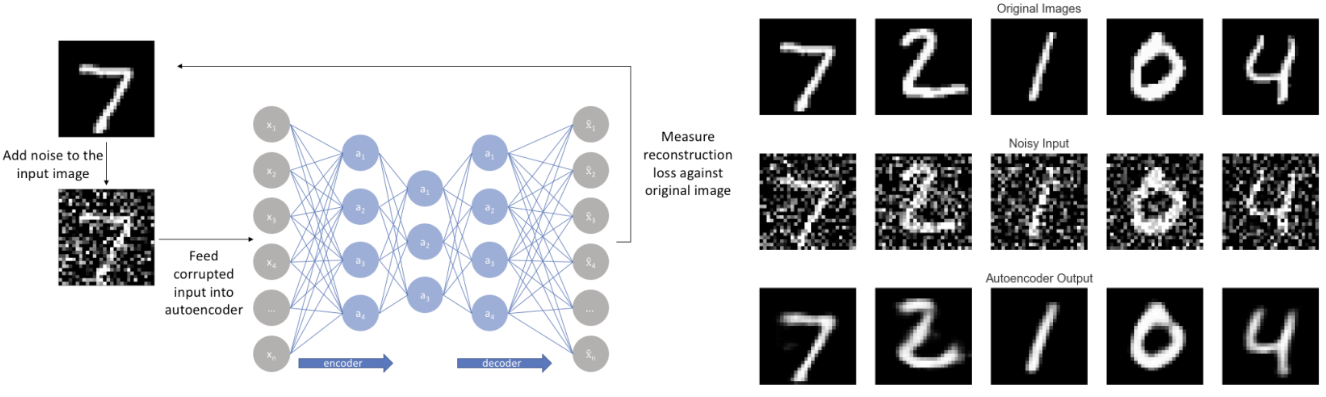
\includegraphics[width=\textwidth]{pic/DAE result on MNIST.png} 
    \end{center}
\end{frame}

\begin{frame}{AE’s: Denoising Autoencoders (It Isn’t Lazy Network!)}
    \begin{itemize}
        \item DAEs won’t simply memorize the inputs and outputs (More robustness)
        \item Intuitively, a DAE learns a \textcolor{blue}{projection} from a neighborhood of our training data back onto the training data 
    \end{itemize}

    \begin{center}
        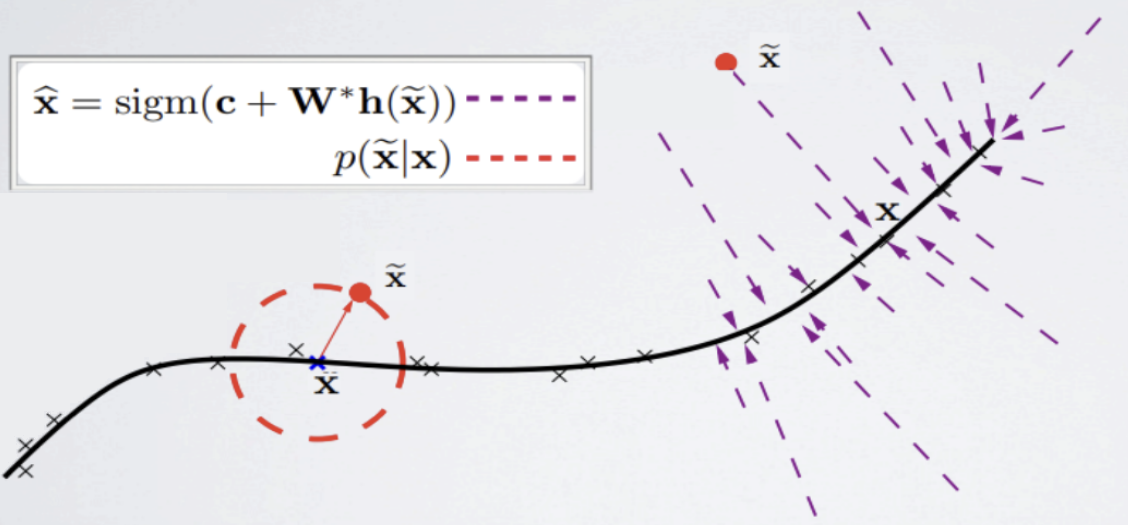
\includegraphics[width=0.7\textwidth]{pic/DAE not lazy1.png}
    \end{center}
\end{frame}

\begin{frame}{AE’s: Denoising Autoencoders (It Isn’t Lazy Network!)}
    \begin{itemize}
        \item DAEs won’t simply memorize the inputs and outputs (More robustness)
        \item Intuitively, a DAE learns a \textcolor{blue}{projection} from a neighborhood of our training data back onto the training data 
    \end{itemize}

    \begin{center}
        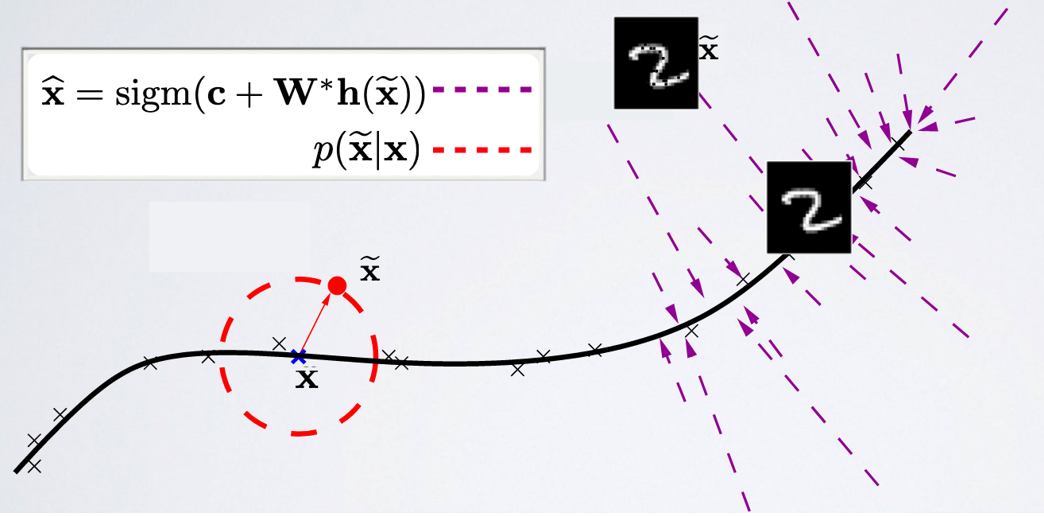
\includegraphics[width=0.65\textwidth]{pic/DAE not lazy2.png}
    \end{center}
\end{frame}

\begin{frame}{AE’s: Denoising Autoencoders (It Isn’t Lazy Network!)}
    \begin{itemize}
        \item  DAEs won’t simply memorize the inputs and outputs (More robustness)
        \item Intuitively, a DAE learns a \textcolor{blue}{projection} from a neighborhood of our training data back onto the training data 
    \end{itemize}

    \begin{center}
        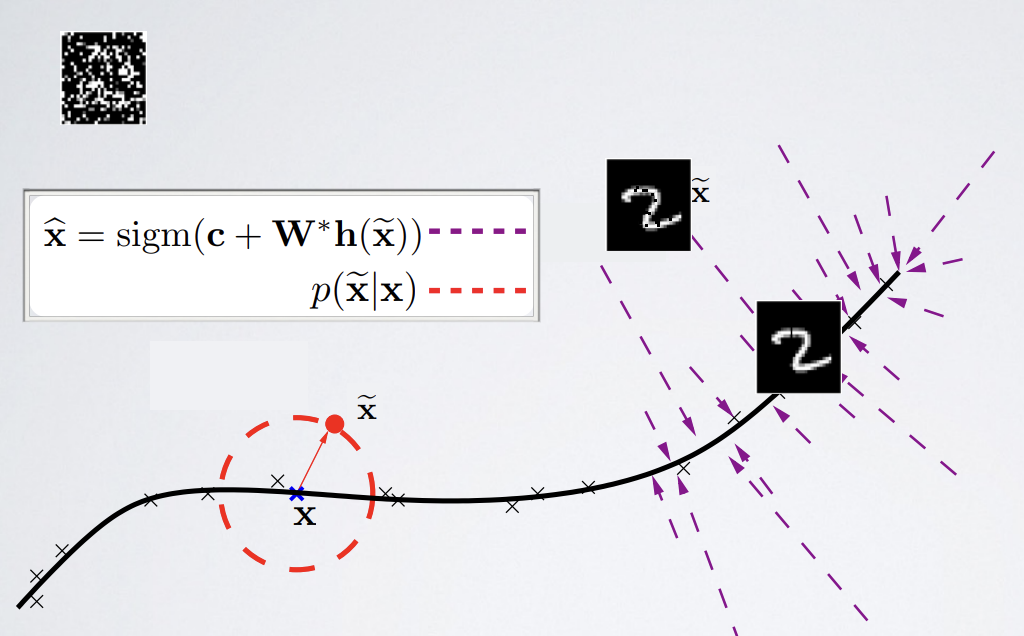
\includegraphics[width=0.6\textwidth]{pic/DAE not lazy3.png}
    \end{center}
\end{frame}

\begin{frame}{AE’s: Contractive Autoencoder (Intuition)}
    \small
    \begin{enumerate}
        \item Contractive autoencoders are explicitly encouraged to learn a manifold through their loss function (Alain and Bengio \textcolor{blue}{2014}).
        \item \textcolor{deepgreen}{Desirable property:} Points close to each other in input space maintain that property in the latent space.
        \item Method to avoid uninteresting solutions
        \item Add an explicit term in the loss that penalizes that solution
        \item We wish to extract features that only reflect variations observed in the training set
        \item We would like to be invariant to other variations
    \end{enumerate}
    
    
    \begin{center}
        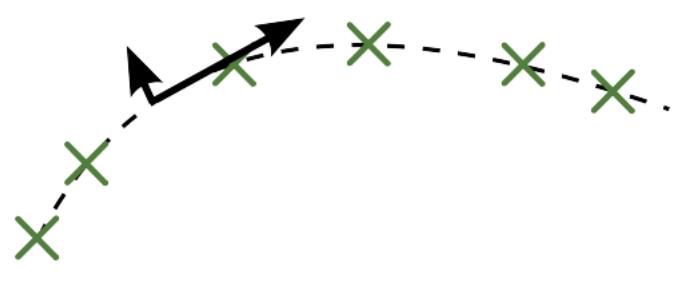
\includegraphics[width=0.45\textwidth]{pic/CAE Intuition1.png} 
    \end{center}
    \vspace{0.4cm}

\end{frame}


\begin{frame}{AE’s: Contractive Autoencoder (Intuition)}
      \begin{center}
        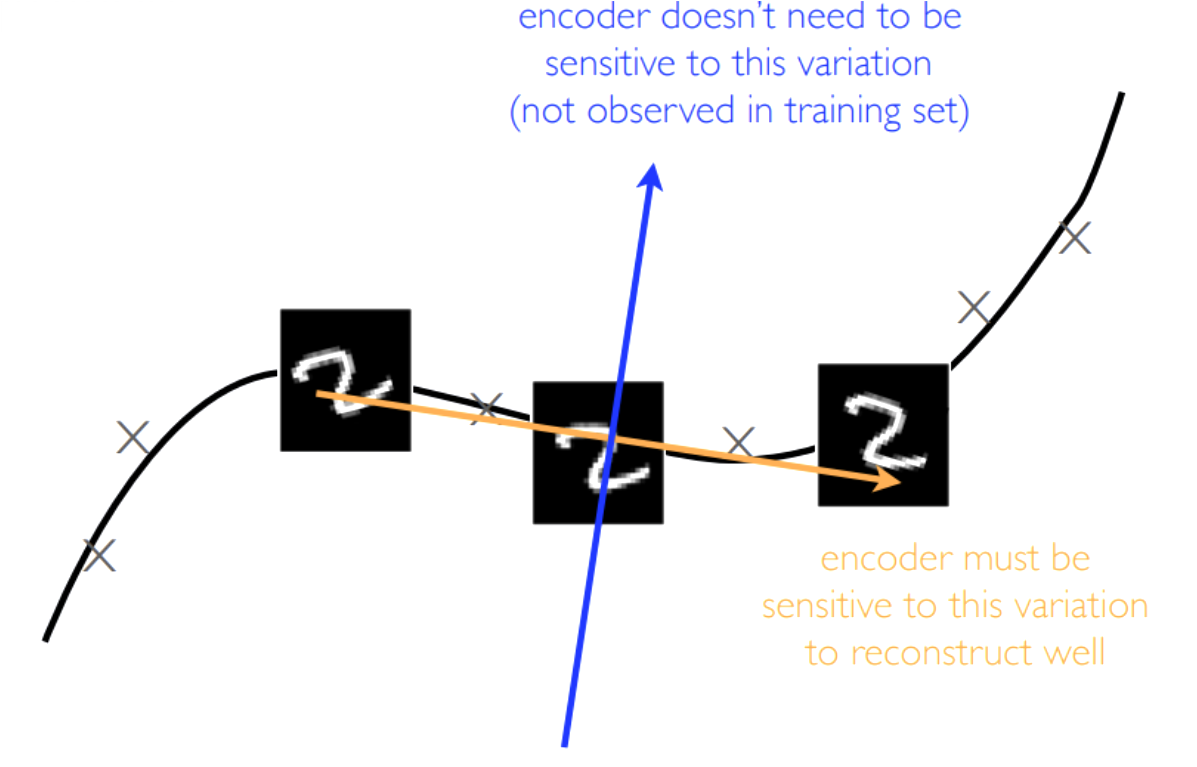
\includegraphics[width=0.7\textwidth]{pic/CAE Intuition2.png} 
    \end{center}
\end{frame}


\begin{frame}{AE’s: Contractive Autoencoder (Details)}
    \scriptsize
    \begin{enumerate}
        \item Contractive autoencoder has an explicit regularizer on \( h = f(x) \), encouraging the derivatives of \( f \) to be as small as possible.
        \item This will be true if \( f(x) = h \) is continuous, has small derivatives.
    \end{enumerate}

    \begin{center}
        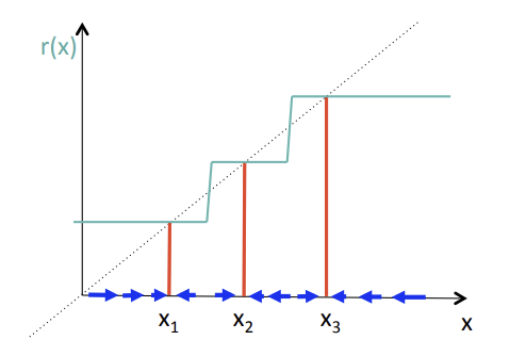
\includegraphics[width=0.2\textwidth]{pic/CAE details1.png}
    \end{center}

    \begin{enumerate}
        \setcounter{enumi}{2} % Continue numbering from 3
        \item We can use the \textcolor{blue}{Frobenius Norm} of the \textcolor{blue}{Jacobian Matrix} as a regularization term:
        
        \[
        \Omega(f, x) = \lambda \left\| \frac{\partial f(x)}{\partial x} \right\|^2_F
        \]
        
        \item These autoencoders are called \textit{contractive} because they contract the neighborhood of input space into a smaller, localized group in latent space.
        
        \item \textbf{\textcolor{red}{Exercise:}} What is the difference between DAE and CAE?
    \end{enumerate}
    
    \vspace{0.4cm}
\end{frame}


\begin{frame}{AE’s: Contractive Autoencoder (Details)}
    \scriptsize

    \begin{itemize}
        \item New loss function:
    \end{itemize}
    
 
        \begin{equation*}
        \ \underbrace{l\left( f\left( x^{( t)}\right)\right)}_{ \begin{array}{l}
        \mathtt{autoencoder\ }\\
        \mathtt{reconstruction}
        \end{array}} +\ \lambda \ \underbrace{\| \nabla _{x^{( t)}} h( x^{( t)} \| _{F}^{2}}_{ \begin{array}{l}
        \mathtt{Jacobian\ of\ }\\
        \mathtt{encoder}
        \end{array}}
        \end{equation*}
        
    \begin{itemize}
        \item where, for binary observations:
    \end{itemize}

            
        \begin{gather*}
        \begin{array}{ c|}
        l\left( f\left( x^{( t)}\right)\right) \ =\ -\Sigma _{k} \ ( x_{k}^{( t)} \ \log\left(\hat{x}_{k}^{( t)}\right) \ +\ \left( 1-x_{k}^{( t)}\right)\log\left( 1-\hat{x}_{k}^{( t)}\right) \ \ \ \Biggr\}\begin{array}{ c }
        \mathtt{encoders\ keeps}\\
        \mathtt{good\ information}
        \end{array}\\
         \\\\
        \| \nabla _{x^{( t)}} h( x^{( t)} \| _{F}^{2} \ =\ \Sigma _{j} \Sigma _{k}\left(\frac{\partial h\left( x^{( t)}\right)_{j}}{\partial x_{k}^{( t)}}\right)^{2} \ \ \ \Biggr\}\begin{array}{ c }
        \mathtt{encoder\ throws}\\
        \mathtt{away\ all\ information}
        \end{array}
        \end{array}\rightarrow \mathtt{\begin{array}{ c }
        \mathtt{encoders\ keep\ only\ }\\
        \mathtt{good\ information}
        \end{array}}\\
        \end{gather*}
\end{frame}




\begin{frame}{Can The Decoder Of AE Be Used For Data Generation?}
    \small
    \begin{itemize}
        \item Autoencoders are effective data compressors but up to now do not yet show \textbf{data generation capabilities}.
        \item We already trained an AE on MNIST; then we use \textbf{random vectors} as input to the Decoder to generate new data.
        \begin{itemize}
            \item Is the \textbf{size} of the bottleneck affecting the \textbf{quality} of the generated sample?
        \end{itemize}
    \end{itemize}
    
    
    % Unified image at the bottom
    \begin{center}
        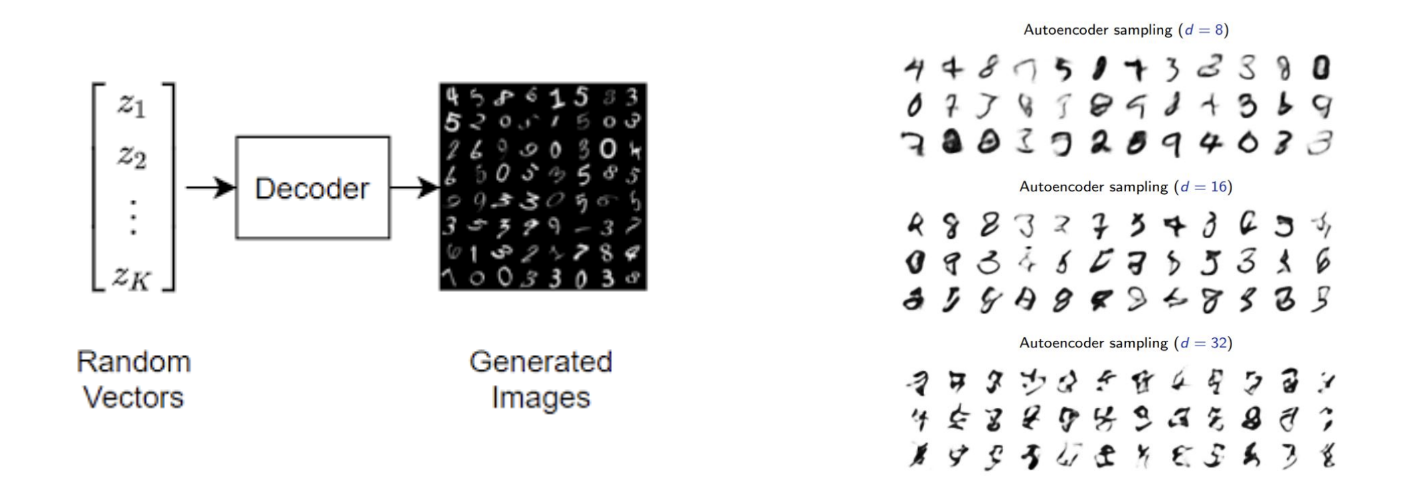
\includegraphics[width=0.9\textwidth]{pic/AE for data generation1.png}
    \end{center}
\end{frame}


\begin{frame}{Can The Decoder Of AE Be Used For Data Generation?}
    Is \textbf{\textcolor{deepred}{any random vector}} we feed into decoder networks results in a valid output?
    \vspace{0.5cm}
    
    % Unified image at the bottom
    \begin{center}
        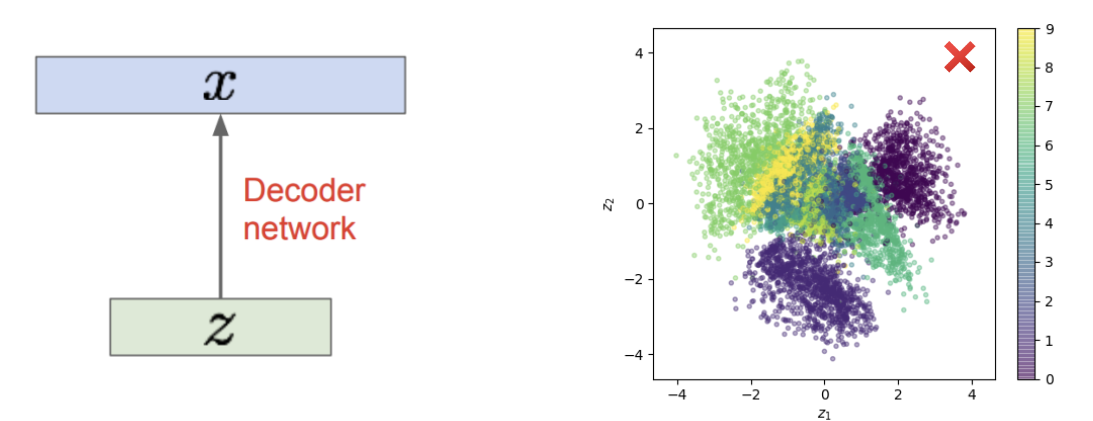
\includegraphics[width=\textwidth]{pic/AE for data generation2.png}
    \end{center}
\end{frame}


\begin{frame}{Can The Decoder Of AE Be Used For Data Generation?}
     \begin{itemize}
            \item \textbf{\textcolor{deepblue}{Latent Variation:}} Varying \textbf{\textit{z}} generates outputs along a learned manifold.
            \item \textbf{\textcolor{deepblue}{Manifold Constraint:}} Data lies within patterns learned from training.
            \item \textbf{\textcolor{deepblue}{Generation:}} Outputs follow the training data distribution.
        \end{itemize}
        
    \vspace{0.5cm}
    
    % Unified image at the bottom
    \begin{center}
        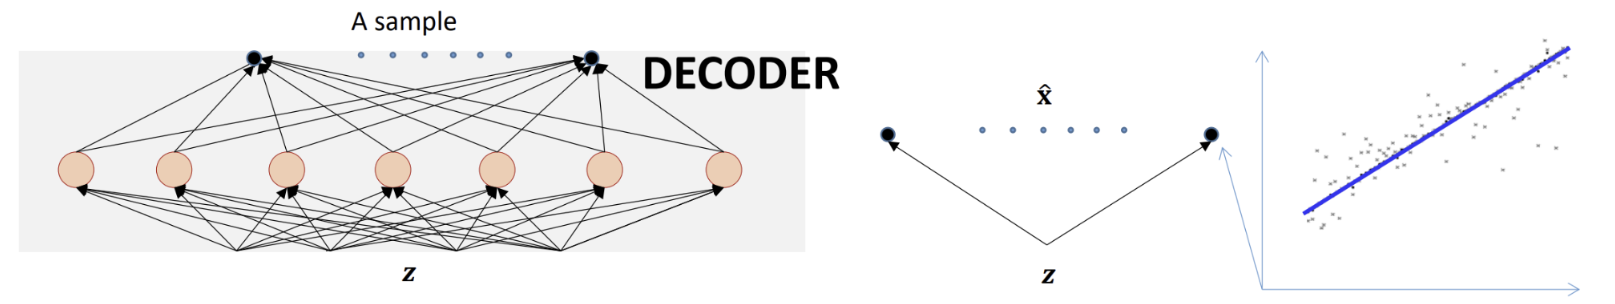
\includegraphics[width=\textwidth]{pic/AE for data generation3.png}
    \end{center}
\end{frame}


\begin{frame}{Latent Space Properties}
    \begin{itemize}
        \item For the generation purpose, we need the latent space to show the following properties:
        \begin{itemize}
            \item \textbf{Continuity:} Similar points in the latent space will be similar after decoding.
            \item \textbf{Completeness:} Samples of the latent space lead to meaningful content after decoding.
        \end{itemize}
    \end{itemize}
\end{frame}

\begin{frame}{Latent Space Properties: Continuity}
      \begin{center}
        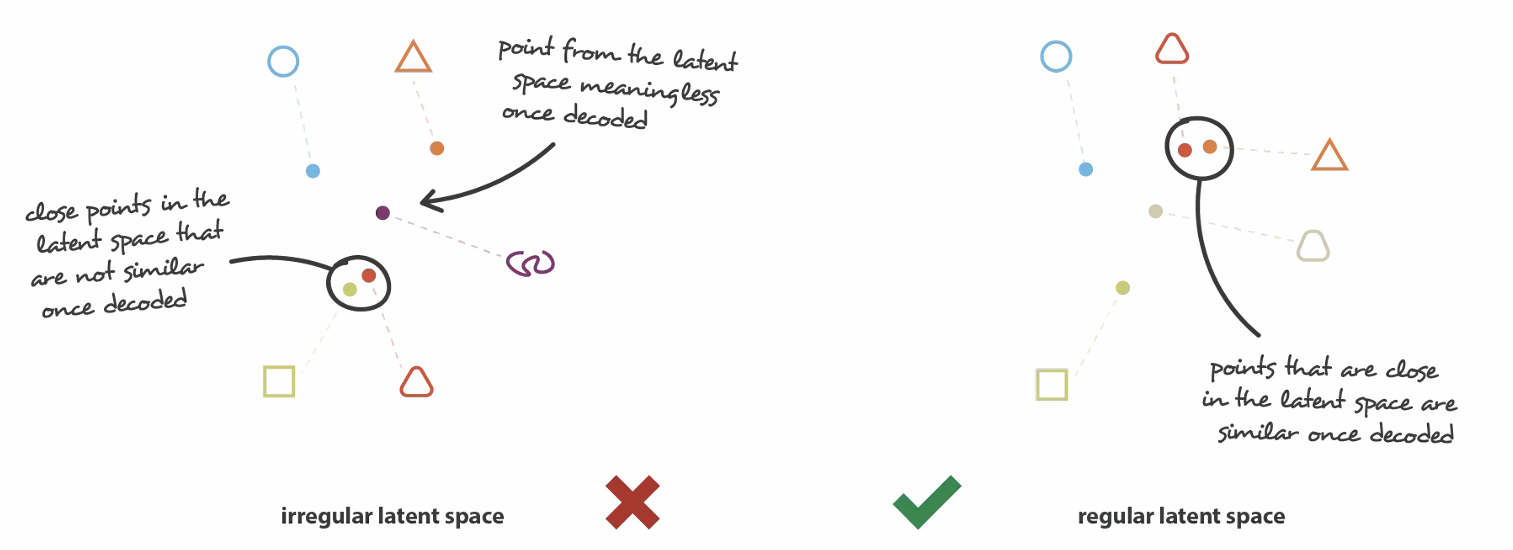
\includegraphics[width=\textwidth]{pic/Latent space property-Continuity.png} 
    \end{center}
\end{frame}


\begin{frame}{Latent Space Properties: Completeness}
      \begin{center}
        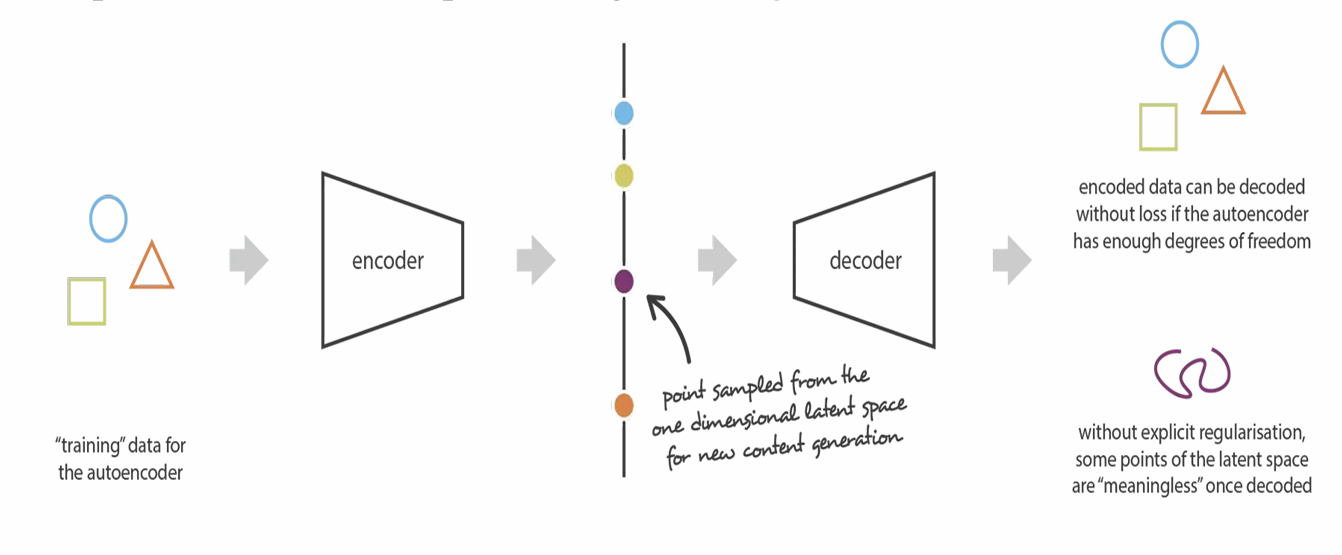
\includegraphics[width=\textwidth]{pic/Latent space property-Completeness.png} 
    \end{center}
\end{frame}

\begin{frame}{AE Latent Space - MNIST}
    \begin{center}
        % Unified image
        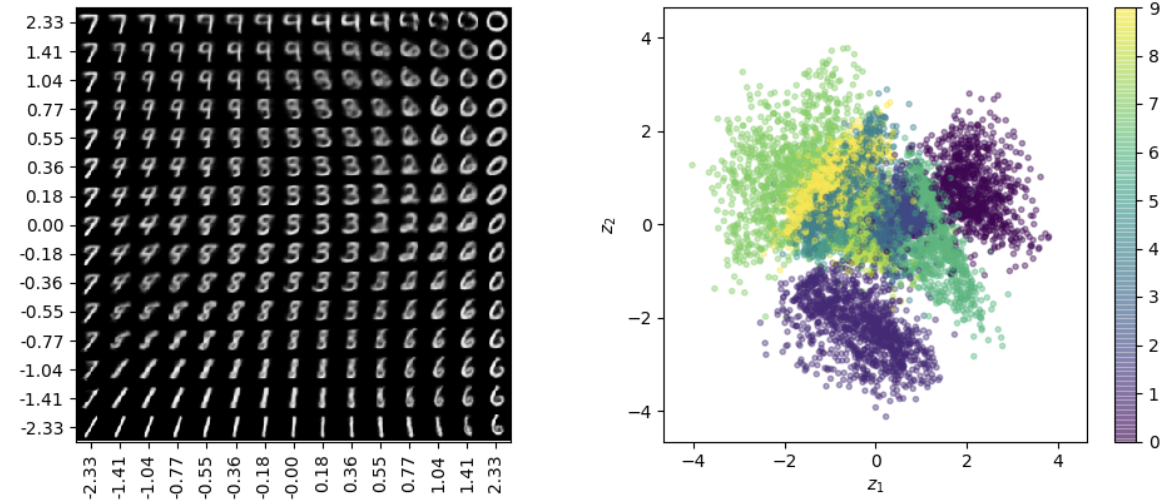
\includegraphics[width=0.9\textwidth]{pic/AE Latent space - MNIST.png}
        {\color{deepred}\textbf{\\ What is the problem?}}
    \end{center}
\end{frame}

\begin{frame}{Latent Variable}
    \begin{itemize}
        \item We define a simple distribution on the latent space, i.e., \( p(z) \) and a decoder network \( p_\theta(\mathbf{x} | \mathbf{z}) \) to map the latent variable to the data space.
    \end{itemize}

    \vspace{0.1cm}

    \begin{equation*}
        p(\mathbf{x}) = \int p(\mathbf{x} | \mathbf{z}) p(\mathbf{z}) \, d\mathbf{z}
    \end{equation*}

    \begin{center}
        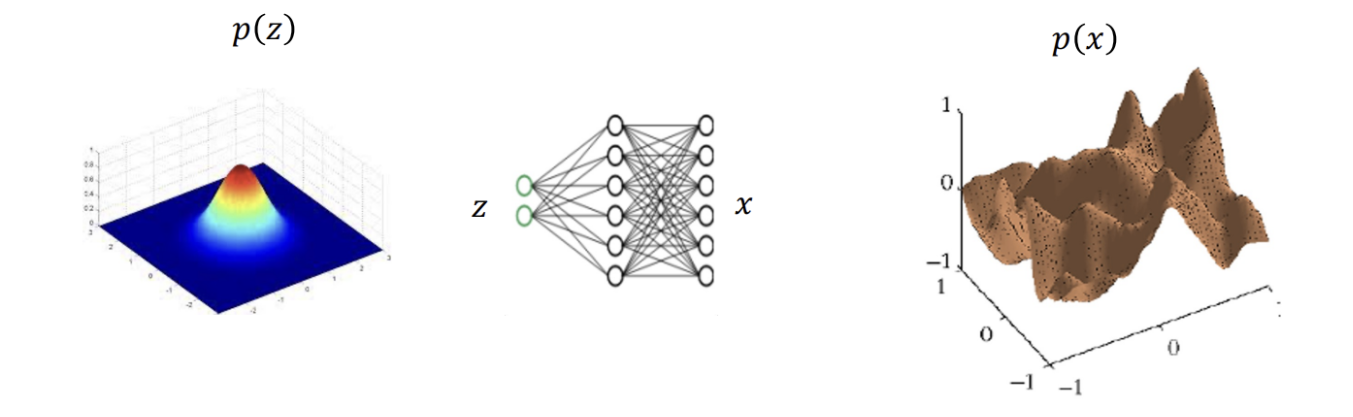
\includegraphics[width=0.8\textwidth]{pic/latent variable.png}
    \end{center}
\end{frame}


\begin{frame}{AE’s: Variational Autoencoder (Intuition)}
    \begin{center}
        \small The key change that they added was that instead of having an encoder that maps points in X to points in Z, VAE’s map points in X to distributions in Z. This allows a point in X to be indirectly mapped to several close neighbour points in Z.
    \end{center}


    \vspace{1.0cm}

    \scriptsize

    
        \begin{equation*}
        \mathbf{Simple\ AE} \ \Biggl\{\text{\ \begin{array}{ c }
        \text{input}\\
        \mathit{x}
        \end{array} \ } \ \ \xrightarrow{\text{\textcolor[rgb]{0.82,0.01,0.11}{Encoding}}\textcolor[rgb]{0.82,0.01,0.11}{\ }} \ \ \text{\ \begin{array}{ c }
        \text{latent\ representation}\\
        \mathit{\ z=e( x)}
        \end{array} \ } \ \ \ \xrightarrow{\text{\textcolor[rgb]{0.29,0.56,0.89}{Decoding}}} \ \text{\ \ \ \begin{array}{ c }
        \text{input\ reconstruction} \ \\
        \mathit{d( z)}
        \end{array}}\Biggr\}
        \end{equation*}
    
    \vspace{0.1cm}
    \hrule
    \vspace{0.1cm}

        \begin{gather*}
        \mathbf{Variational\ AE}\ \Biggl\{\ \begin{array}{c}
        \text{input} \\
        \mathit{x}
        \end{array} \ \xrightarrow{\text{\textcolor[rgb]{0.82,0.01,0.11}{Encoding}}} \ \begin{array}{c}
        \text{latent distribution} \\
        p(z|x)
        \end{array} \ \xrightarrow{\text{\textcolor[rgb]{0.25,0.46,0.02}{Sampling}}} \ \begin{array}{c}
        \text{sampled latent} \\
        \text{representation} \\
        z \sim p(z|x)
        \end{array} \ \xrightarrow{\text{\textcolor[rgb]{0.29,0.56,0.89}{Decoding}}} \ \begin{array}{c}
        \text{input reconstruction} \\
        d(z)
        \end{array} \ \Biggr\}
        \end{gather*}
        
    
\end{frame}


\begin{frame}{AE’s: Variational Autoencoder (Big Picture)}
    \begin{center}
        \small The key change that they added was that instead of having an encoder that maps points in X to points in Z, VAE’s map points in X to distributions in Z. This allows a point in X to be indirectly mapped to several close neighbour points in Z.

        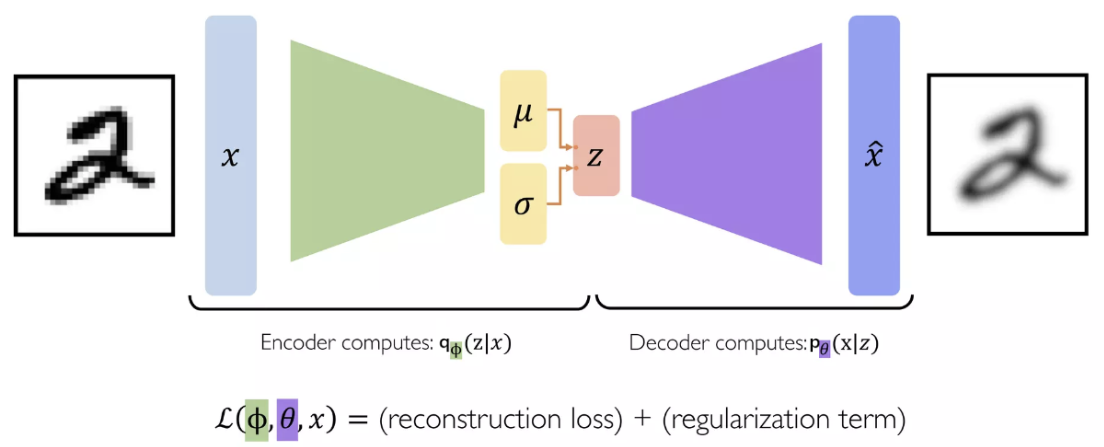
\includegraphics[width=0.9\textwidth]{pic/VAE big picture.png}

    \end{center}
  
    
\end{frame}



\begin{frame}{AE's: Variational Autoencoder (Details)}
    \begin{center}
        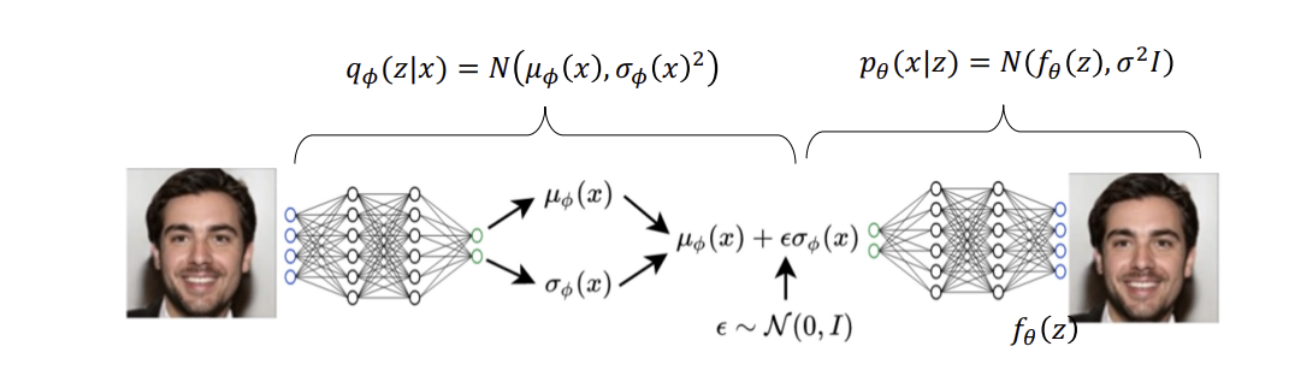
\includegraphics[width=0.9\textwidth]{pic/VAE details1.png}
    \end{center}
    \scriptsize
    \begin{equation*}
        \textbf{VAE loss: } \mathcal{L}(x, \theta, \phi) = 
        \underbrace{
            \| x^{(i)} - \hat{x}^{(i)} \|^2
        }_{\substack{
            \text{\textcolor[rgb]{0.29,0.56,0.89}{reconstruction loss}} \\ 
            \\
            \\
            \downarrow\\
            \\
            f_{\theta}(z) = f_{\theta} \big( \mu_{\phi}(x^{(i)}) + \epsilon \sigma_{\phi}(x^{(i)}) \big)
        }}
        + 
        \underbrace{
            KL\left( q_{\phi}(z | x^{(i)}) \parallel \mathcal{N}(0, I) \right)
        }_{\substack{
            \text{\textcolor[rgb]{0.82,0.01,0.11}{regularization term}} \\ 
            \\
            \downarrow\\
            \\
            \text{Common choice of prior on} \\
            \text{the latent distribution.}
        }}
    \end{equation*}

\end{frame}

\begin{frame}{AE's: Variational Autoencoder (Details)}
    \begin{itemize}
        \item Encourage encodings to be evenly distributed around the center of the latent space
        \item Penalize the network when it tries to memorize data
    \end{itemize}
    
    \begin{center}
        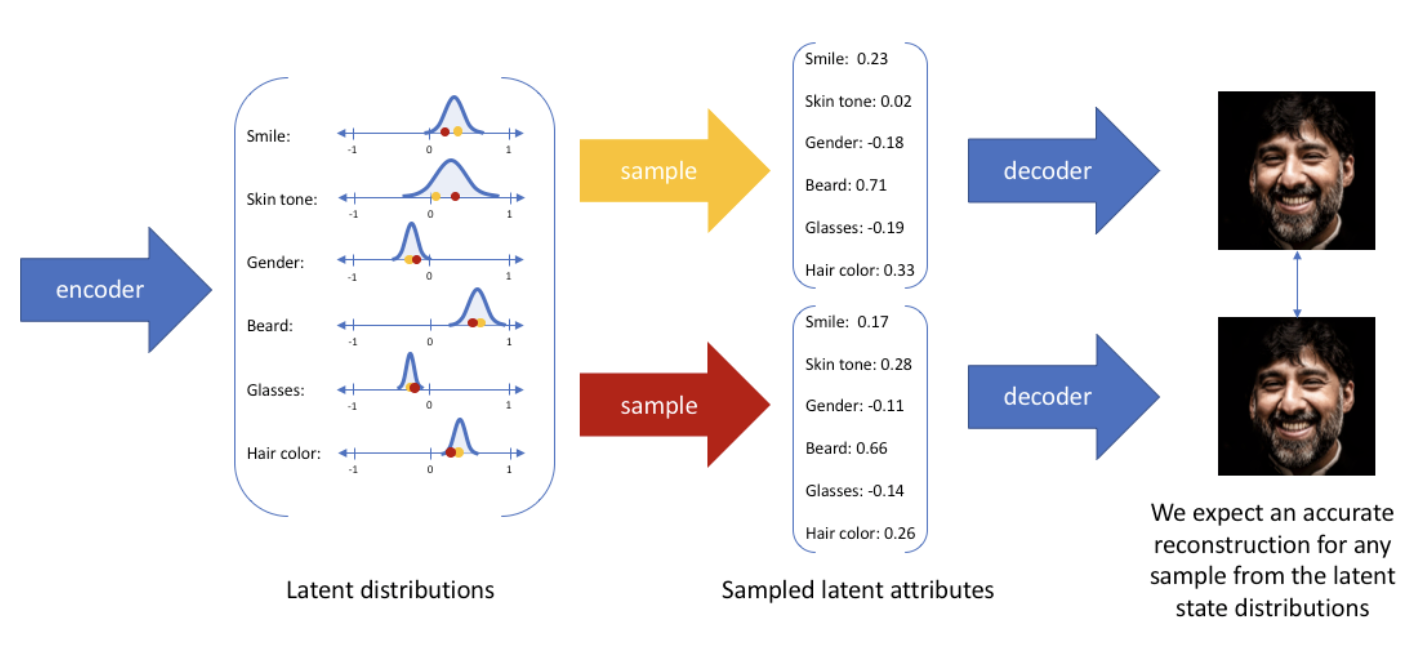
\includegraphics[width=0.8\textwidth]{pic/VAE details2.png}
        
            \vfill
    \hspace*{-1\textwidth}{\scriptsize Image: \href{https://github.com/Shakib-IO/Variational_Autoencoder_MNIST_Dataset}{Source}}


    \end{center}
\end{frame}

\begin{frame}{AE's: Variational Autoencoder (Details)}
    \begin{center}
        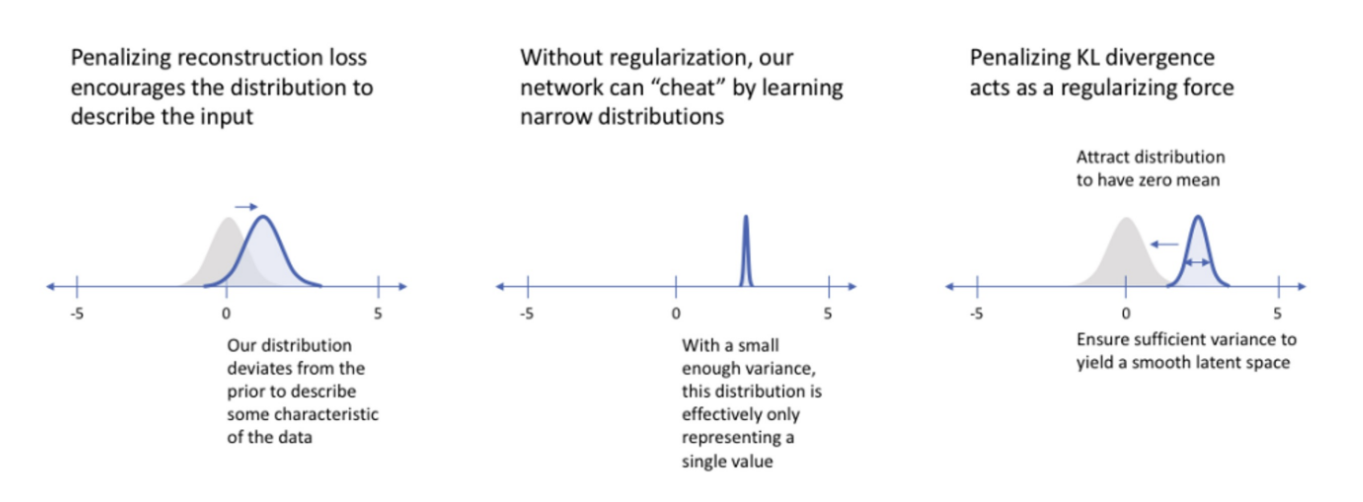
\includegraphics[width=0.95\textwidth]{pic/VAE details3.png}
    \end{center}
    The VAE objectives arranges data on a compact manifold (we can sample from) in a continuous smooth way.

\end{frame}


\begin{frame}{AE other Applications: Anomaly Detection}
    \begin{columns}
        % Left Image
        \begin{column}{0.5\textwidth}
            \begin{center}
                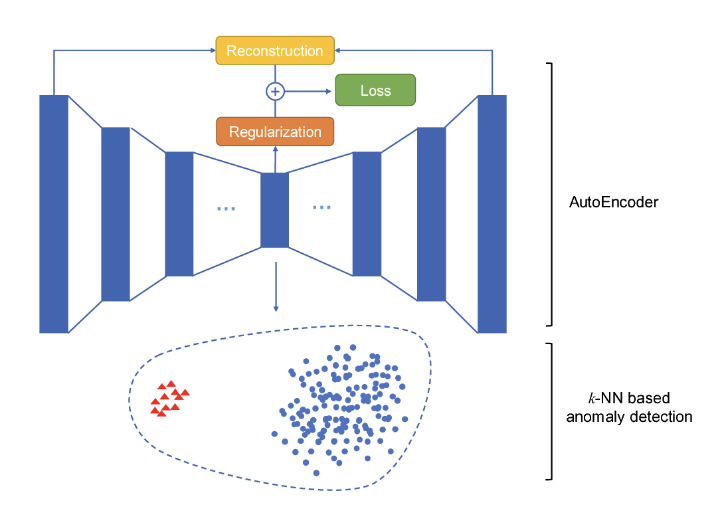
\includegraphics[width=\textwidth]{pic/AE other app anomaly detection1.png}
            \end{center}
        \end{column}

        % Right Image
        \begin{column}{0.5\textwidth}
            \begin{center}
                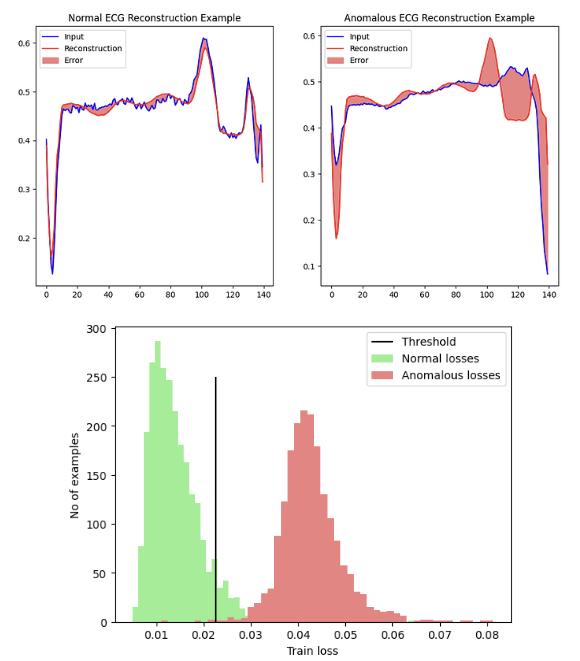
\includegraphics[width=0.8\textwidth]{pic/AE other app anomaly detection2 .png}
            \end{center}
        \end{column}
    \end{columns}
\end{frame}

\begin{frame}{AE other Applications: Image Colorization}
      \begin{center}
        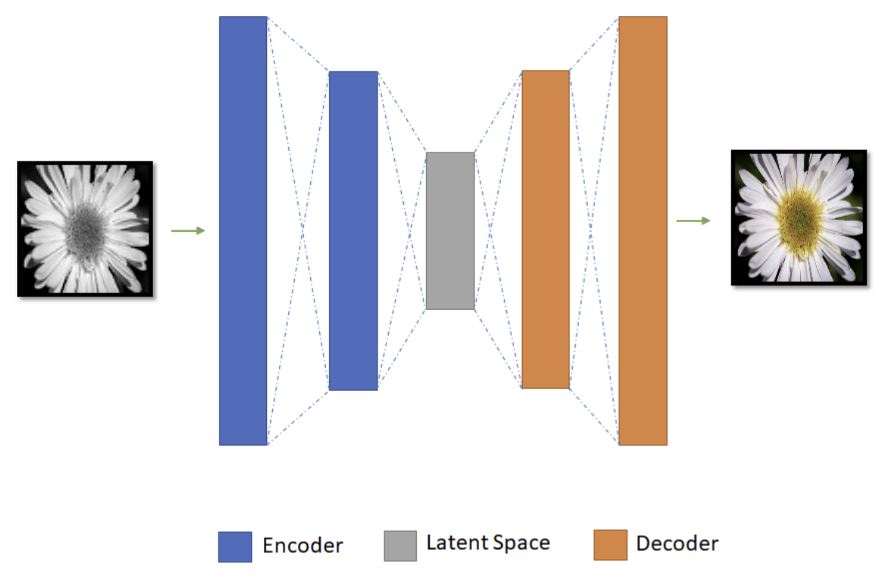
\includegraphics[width=0.7\textwidth]{pic/AE other app colorization.png} 
    \end{center}
\end{frame}


\begin{frame}{AE other Applications: Fake Lough}
      \begin{center}
        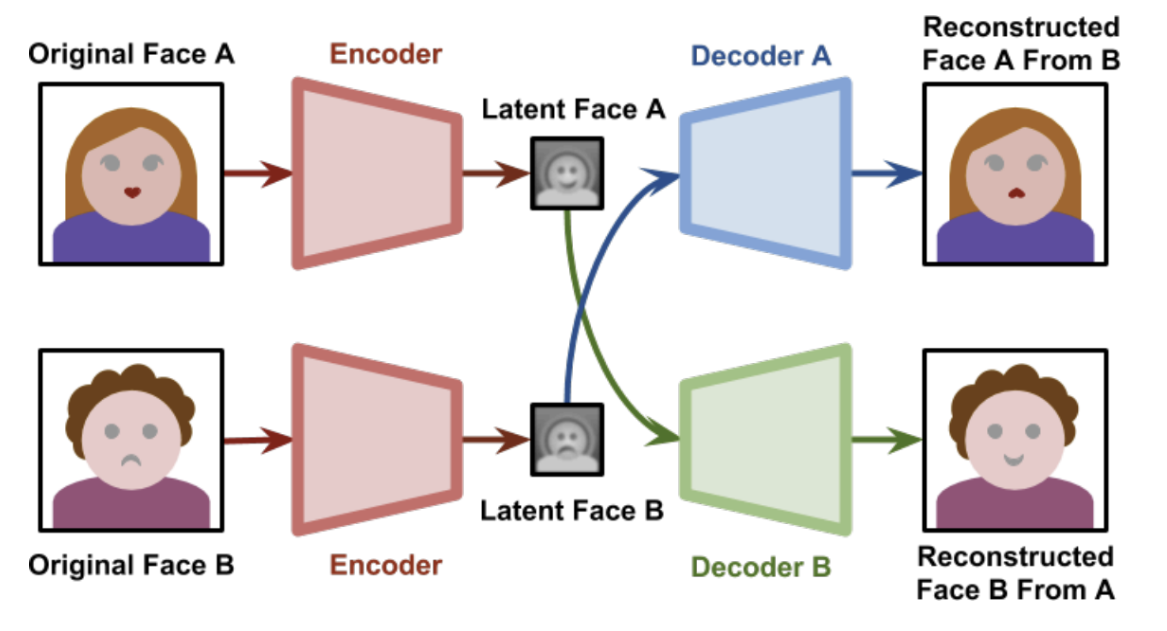
\includegraphics[width=0.8\textwidth]{pic/AE other app Fake Lough.png} 
    \end{center}
\end{frame}






\section{References}

\begin{frame}[allowframebreaks]
    \bibliography{ref}
    \bibliographystyle{ieeetr}
    \nocite{*} % used here because no citation happens in slides
    \small
    \textbf{Slides by: Amirhossein Izadi}
    \begin{itemize}
        \item F.-F. Li, J. Wu, and R. Gao, “CS231n” Lecture slides, 2024, Stanford 
        \item A. Amini, “6s191” Lecture slides, 2024, MIT. 
        \item M. Soleymani, “Deep Learning” Lecture slides, 2024, Sharif University of Technology.
        \item H. Beigy, “Deep Learning” Lecture slides, 2022, Sharif University of Technology.
        \item S. Levine, “CS W182/282A” Lecture slides, 2024, UC Berkeley 
        \item Y. Maziane, “Diffusion models: Seek of information and structure in latent space,” 2022, University of Liège.
        \item G. Buzzard, “Mathematical Aspects of Neural Networks” Lecture slides, 2019, Purdue University.
    \end{itemize}
\end{frame}


\begin{frame}
    \begin{center}
        {\Huge Any Questions?}
    \end{center}
\end{frame}

\end{document}